\Chapter{RÉSULTATS THÉORIQUES}\label{sec:Theme2}

Après avoir déterminé des expressions analytiques pour les différentes fonctions étudiées, il est essentiel d'analyser les résultats obtenus afin de vérifier leur validité et leur cohérence avec le modèle théorique. 

Pour évaluer le comportement des fonctions obtenues, il est nécessaire de se placer dans un cadre particulier du processus étudié. En se basant sur la définition du processus \acs{CIR} (\ref{cir_eq}) et du problème de premier passage (\ref{fpt_definition}), les paramètres suivants sont considérés pour l'ensemble des analyses:

\begin{itemize}
    \item Vitesse de retour à la moyenne du \acs{CIR}: $a=0.1$
    \item Niveau moyen du \acs{CIR}: $b=0.9$
    \item Volatilité instantanée du \acs{CIR}: $\sigma=1$
    \item Frontière supérieure pour le \acs{TPP}: $c=1$
\end{itemize}

\section{Diffusion pure}

D'abord, les résultats trouvés pour le processus de diffusion pure sont abordés.

\subsection{Fonction Génératrice des Moments}

\paragraph{Visualisation}\phantom{}\\
Pour commencer, il convient de valider le comportement de la \acl{FGM} $M(x;\alpha)$ définie par (\ref{fgm}), (\ref{sol_fgm}) et (\ref{fgm_constants}). À cet effet, il faut tracer son évolution sur l'intervalle $[0, c]$ pour plusieurs valeurs du paramètre $\alpha \in \{1, 2, 5, 10\}$. 


\begin{figure}[htb]
    \centering
    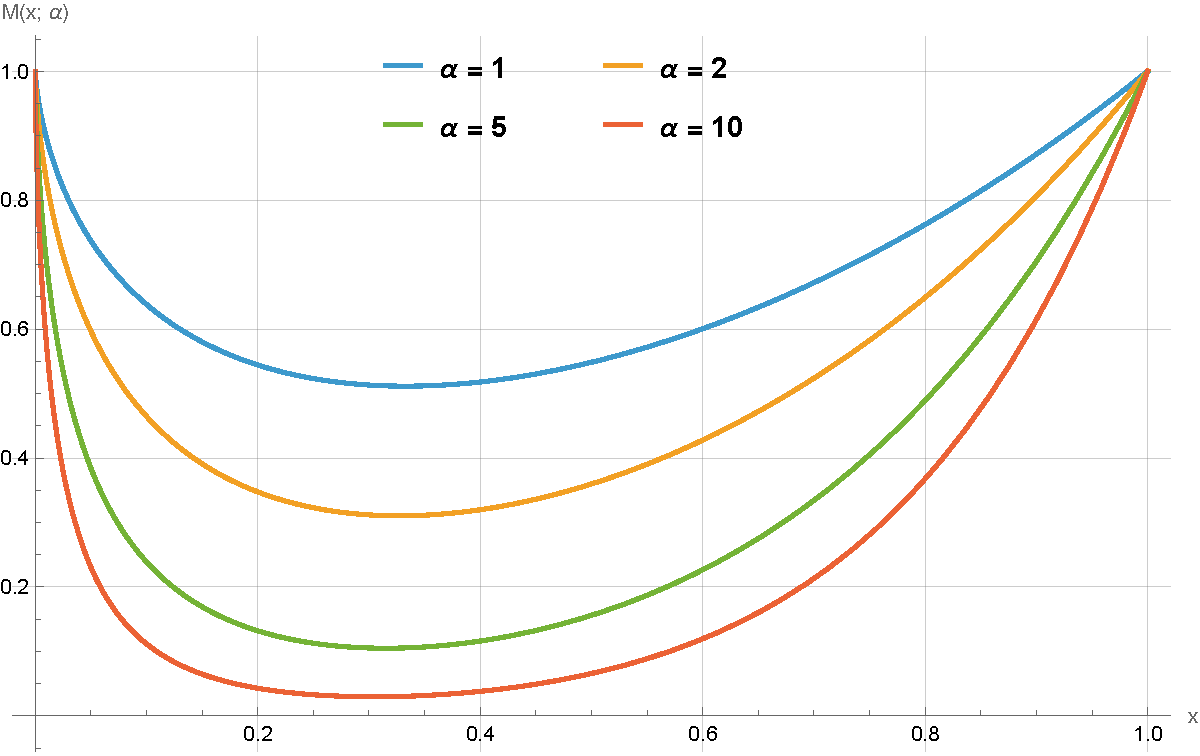
\includegraphics[width=0.5\linewidth]{img/validation/fgm.pdf}
    \caption{Visualisation de la \acl{FGM} $M(x;\alpha)$}\label{fig:FGMVisualisation}
\end{figure}
\FloatBarrier\paragraph{Analyse}\phantom{}\\
Il est important de souligner les points suivants:
\begin{itemize}
    \item Les conditions aux limites $M(0; \alpha) = M(c; \alpha) = 1$ sont respectées;
    \item Puisque $\alpha$ est par définition un paramètre positif (\ref{fgm}), la fonction est bien comprise dans l'intervalle $(0, 1)$, car elle correspond à l'exponentielle d'un nombre négatif; 
    \item Par ailleurs, et pour la même raison, lorsque $\alpha$ augmente, la fonction diminue.
\end{itemize}

L'expression obtenue pour la \acl{FGM} est ainsi validée. 


\subsection{Fonction Temps Moyen}

\paragraph{Visualisation}\phantom{}\\
Ensuite, il est nécessaire de valider le comportement de la fonction Temps Moyen $m(x)$ définie par (\ref{mean}), (\ref{sol_mean}) et (\ref{mean_constants}). La fonction est donc tracée pour différentes valeurs des paramètres $a,\;\forall\;a\in\{0.1,0.2,0.4\}$ et $\sigma,\;\forall\;\sigma\in\{1,\sqrt{2},2\}$.


\begin{figure}[htb]
    \centering
    \begin{subfigure}{0.45\linewidth}
        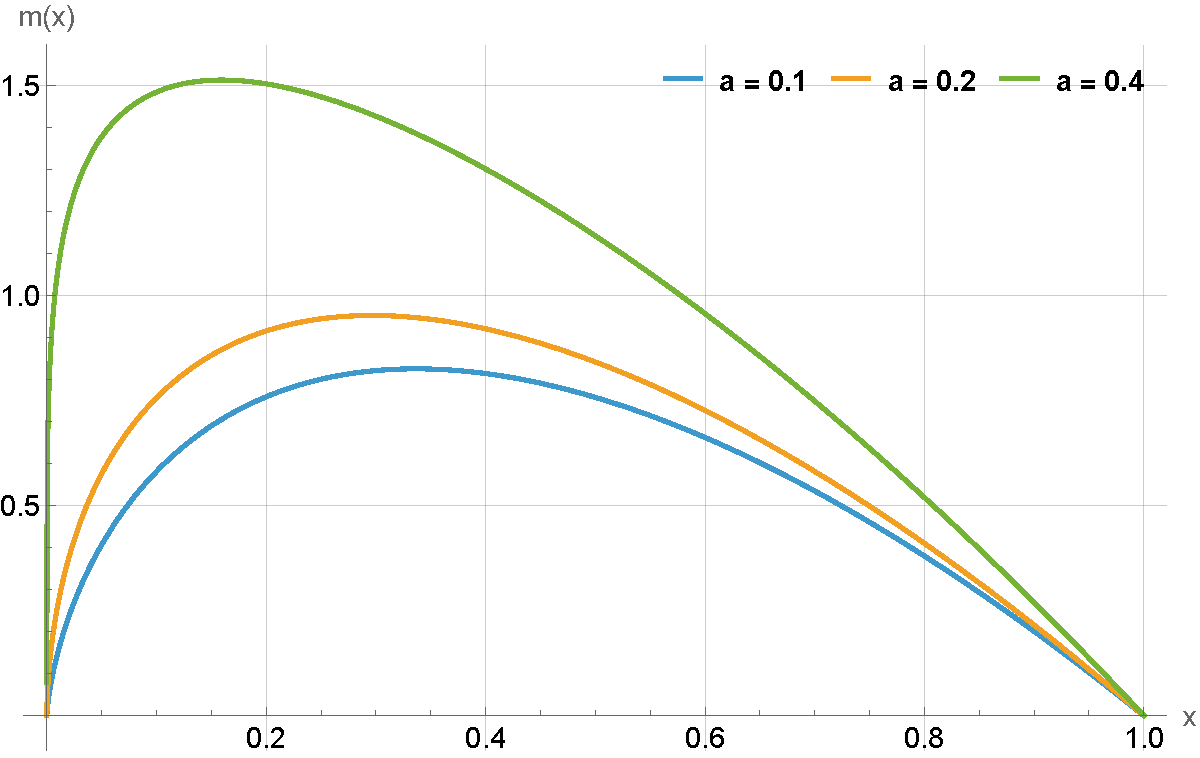
\includegraphics[width=\linewidth]{img/validation/Mean/mean_a.pdf}
        \caption{Sensibilité de la vitesse $a$}\label{fig:Mean_a_visualisation}
    \end{subfigure}
    \hfill
    \begin{subfigure}{0.45\linewidth}
        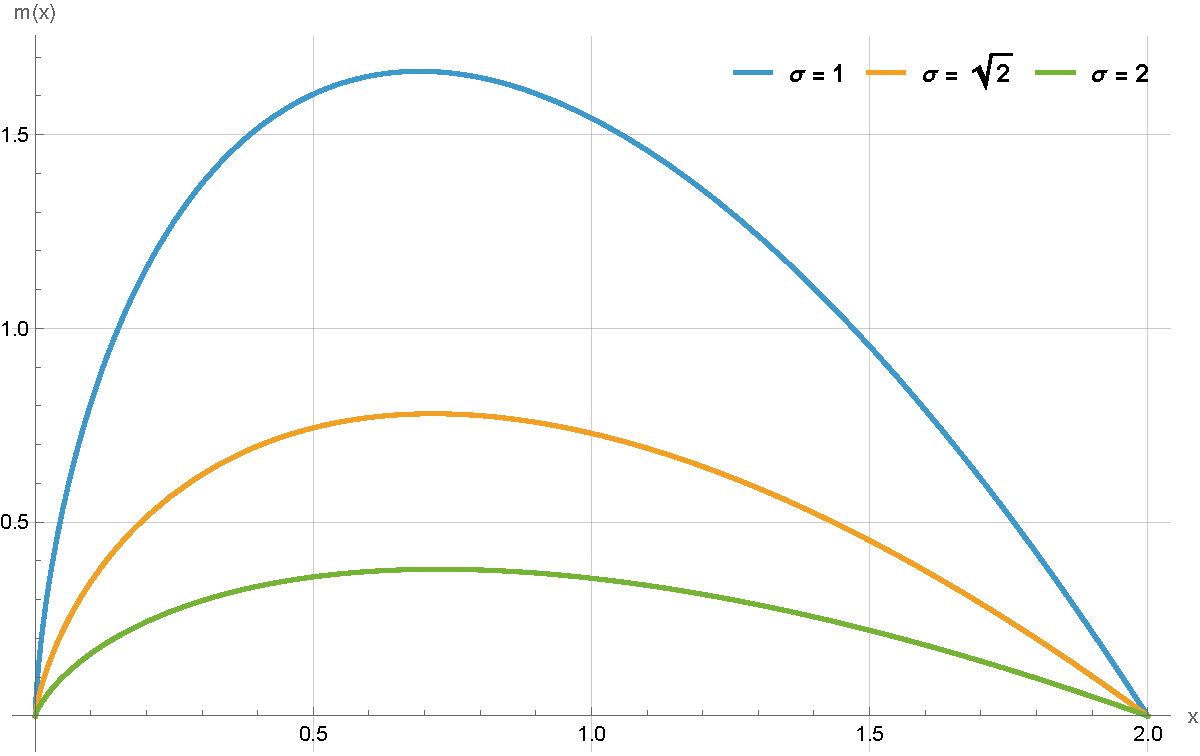
\includegraphics[width=\linewidth]{img/validation/Mean/mean_sigma.pdf}
        \caption{Sensibilité de la volatilité infinitésimale $\sigma$}\label{fig:Mean_sigma_visualisation}
    \end{subfigure}
    \caption{Visualisation de la fonction Temps Moyen $m(x)$}\label{fig:MeanVisualisation}
\end{figure}
\FloatBarrier\paragraph{Analyse}\phantom{}\\
Il est important de noter les points suivants concernant toutes les valeurs différentes des paramètres:
\begin{itemize}
    \item Les conditions aux limites $m(0)=m(c)=0$ sont respectées;
    \item Cette fonction représente un \textit{temps moyen de premier passage}, elle doit donc être positive pour toute valeur de $x$ dans $[0,c]$;
    \item Une augmentation de la vitesse de retour $a$ entraîne une hausse du temps moyen de sortie de l'intervalle. En effet, plus la force de rappel vers la moyenne est forte (i.e., $a$ élevé), plus une déviation significative et peu probable est nécessaire pour franchir les bornes de l'intervalle;
    \item À l'inverse, une augmentation de la volatilité infinitésimale $\sigma$ diminue le temps moyen de sortie. Cela s'explique naturellement: des fluctuations plus intenses accroissent la probabilité de quitter rapidement l'intervalle.
\end{itemize}

L'expression obtenue pour la fonction de temps moyen de premier passage est ainsi validée.

\subsection{Fonction Aire Moyenne}

\paragraph{Visualisation}\phantom{}\\
Par ailleurs, la même démarche de validation est effectuée pour la fonction Aire Moyenne $A(x)$ définie par (\ref{area}), (\ref{sol_area}) et (\ref{area_constants}).

\begin{figure}[htb]
    \centering
    \begin{subfigure}{0.45\linewidth}
        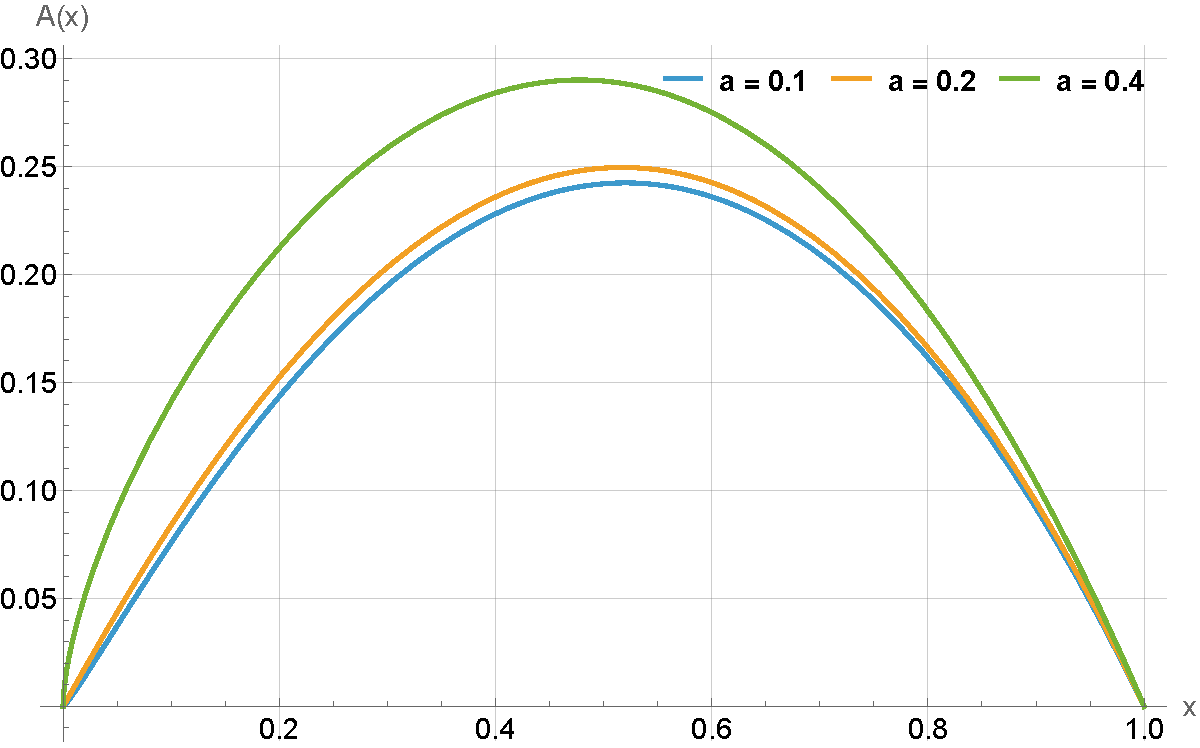
\includegraphics[width=\linewidth]{img/validation/Area/area_a.pdf}
        \caption{Sensibilité de la vitesse $a$}\label{fig:Area_a_visualisation}
    \end{subfigure}
    \hfill
    \begin{subfigure}{0.45\linewidth}
        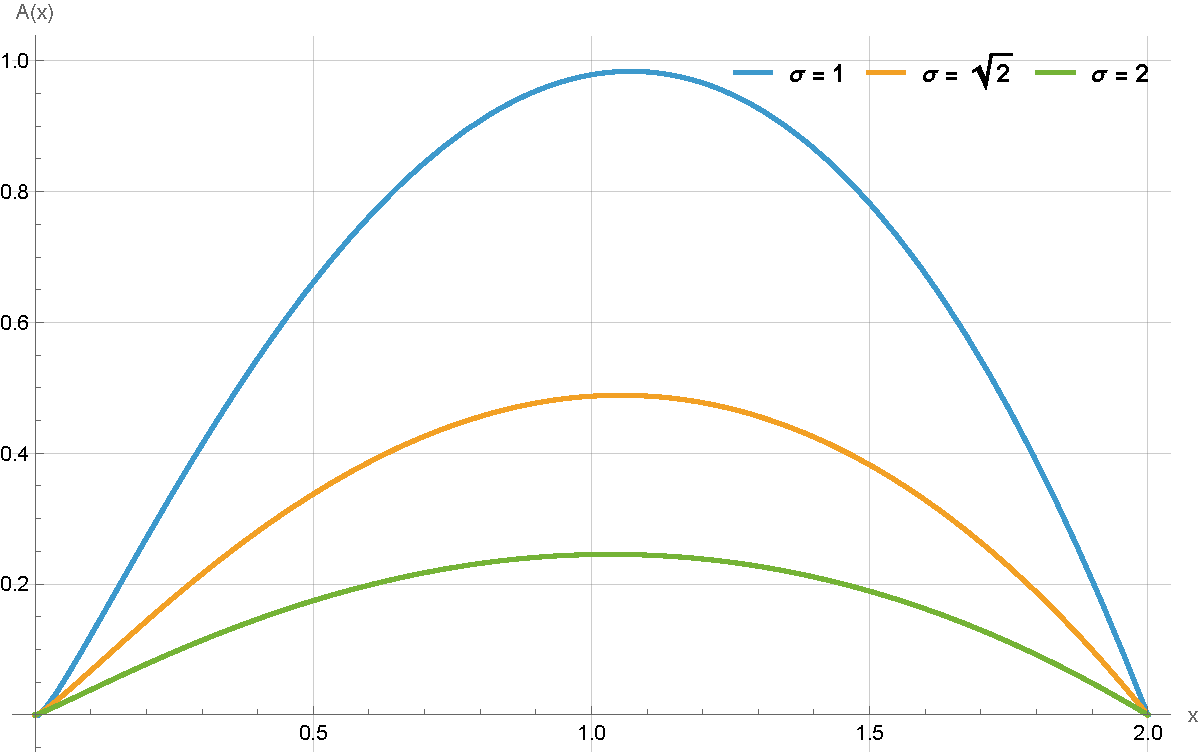
\includegraphics[width=\linewidth]{img/validation/Area/area_sigma.pdf}
        \caption{Sensibilité de la volatilité infinitésimale $\sigma$}\label{fig:Area_sigma_visualisation}
    \end{subfigure}
    \caption{Visualisation de la fonction Aire Moyenne $A(x)$}\label{fig:AreaVisualisation}
\end{figure}
\FloatBarrier\paragraph{Analyse}\phantom{}\\
Il convient de souligner les points suivants:
\begin{itemize}
    \item Les conditions aux limites $A(0)=A(c)=0$ sont respectées;
    \item Cette fonction représente une \textit{aire moyenne} sous un processus positif, elle doit donc être positive pour toute valeur de $x$ dans $[0,c]$;
    \item Une augmentation de la vitesse de retour $a$ entraîne une augmentation de l'aire moyenne sous le processus avant la sortie de l'intervalle. En effet, une force de rappel plus intense maintient le processus autour de sa moyenne plus longtemps, retardant la sortie et augmentant ainsi l'accumulation totale;
    \item À l'inverse, une augmentation de la volatilité infinitésimale $\sigma$ réduit l'aire moyenne. Des fluctuations plus fortes rendent les sorties plus précoces, limitant la durée pendant laquelle le processus peut contribuer à l'intégrale.
\end{itemize}

L'expression obtenue pour la fonction Aire Moyenne est ainsi validée.

\subsection{Commande Optimale Stochastique}

Enfin, il est nécessaire de valider les expressions obtenues dans le cadre des trois problèmes de commande optimale étudiés. Pour cela, il convient de tracer la fonction valeur $F(x)$ ainsi que le contrôle optimal $u^*(x)$, et s'il est possible, pour plusieurs valeurs des différents paramètres des coûts. Afin d'isoler l'influence d'un paramètre lors de l'analyse, les autres seront fixés à $1$.

\subsubsection{Problème linéarisable 1 \textemdash~P1}\phantom{}\\
Le problème (\ref{p1}) est considéré. D'un côté, les fonctions $r(x)$, $b(x)$ et $q(x)$ sont définies en (\ref{p1}). D'un autre côté, la fonction valeur $F(x)$ est définie par (\ref{sol_control_1},~\ref{control_constants}) et le contrôle optimal est défini par (\ref{optimal_control_1}). D'abord, tous les paramètres de coûts sont: $\rho=\beta=\kappa=1$.
\begin{figure}[htb]
    \centering
    \begin{subfigure}{0.45\linewidth}
        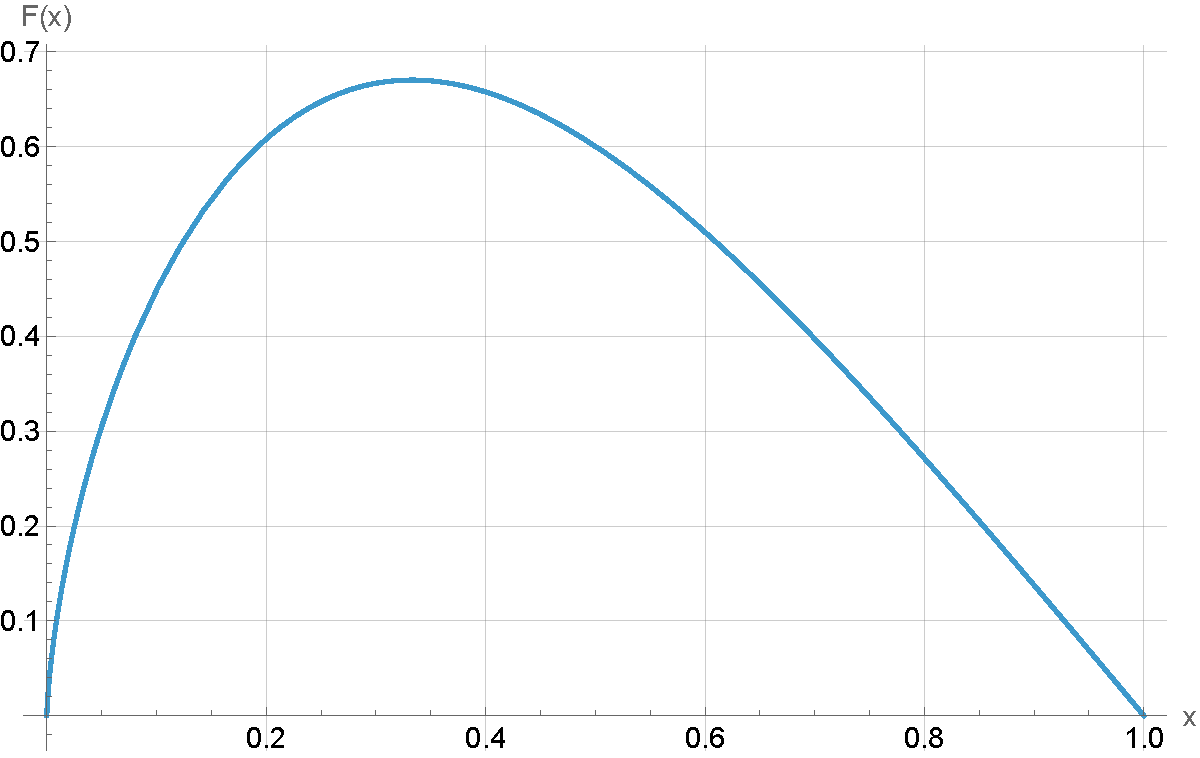
\includegraphics[width=\linewidth]{img/validation/P1/p1_value.pdf}
        \caption{P1 \textemdash~Fonction Valeur $F(x)$}\label{fig:ValueVisualisation1}
    \end{subfigure}
    \hfill
    \begin{subfigure}{0.45\linewidth}
        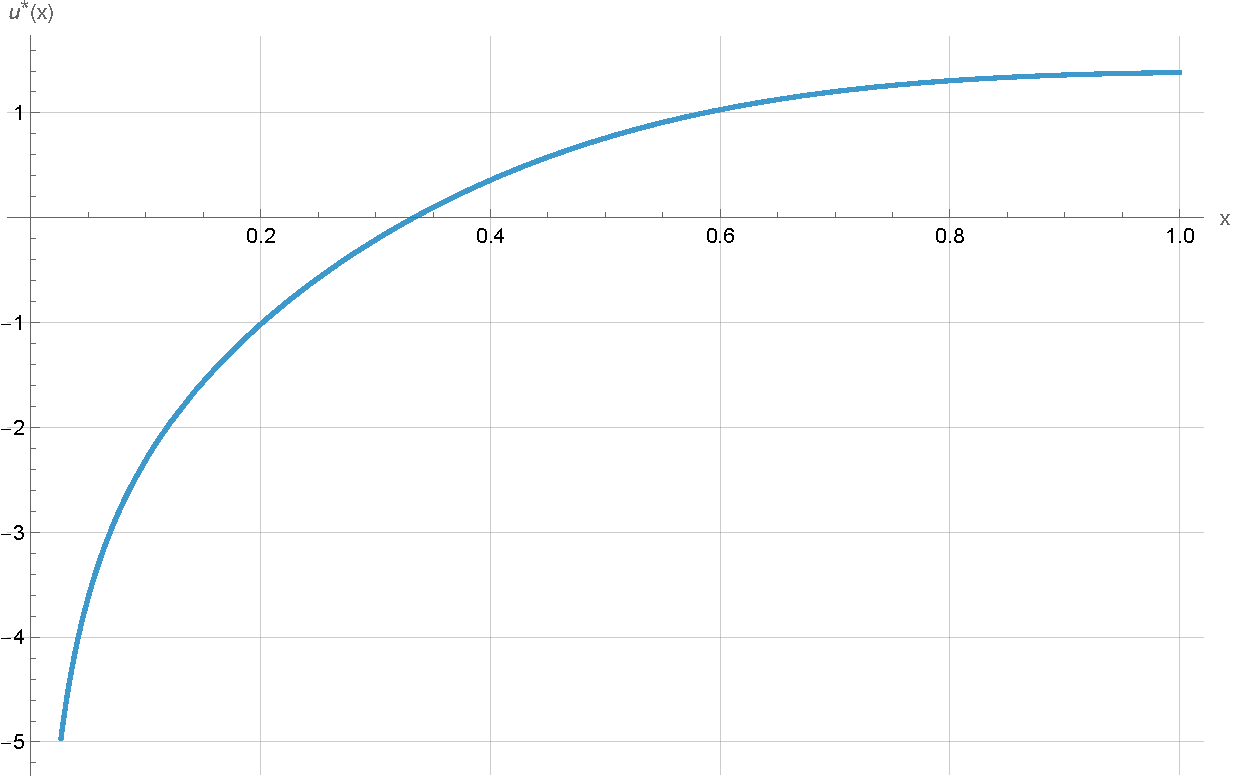
\includegraphics[width=\linewidth]{img/validation/P1/p1_control.pdf}
        \caption{P1 \textemdash~Contrôle Optimal $u^*(x)$}\label{fig:ControlVisualisation1}
    \end{subfigure}
    \caption{P1 \textemdash~Visualisation de la fonction valeur et du contrôle optimal}\label{fig:ValueControlComparison1}
\end{figure}\FloatBarrier De plus, il est intéressant d'analyser la sensibilité de ces fonctions par rapport à la variation des coûts. Les différentes valeurs des paramètres suivants sont évaluées:
\begin{itemize}
    \item Paramètre du coût immédiat $\rho,\;\forall\;\rho\in\{1,2,3,4\}$
    \item Paramètre du coût de contrôle $\beta,\;\forall\;\beta\in\{1,2,3,4\}$
    \item Paramètre du poids pénalisant l'intensité du contrôle $\kappa,\;\forall\;\kappa\in\{1,2,3,4\}$
\end{itemize}
\begin{figure}[htb]
    \centering
    \begin{subfigure}{0.45\linewidth}
        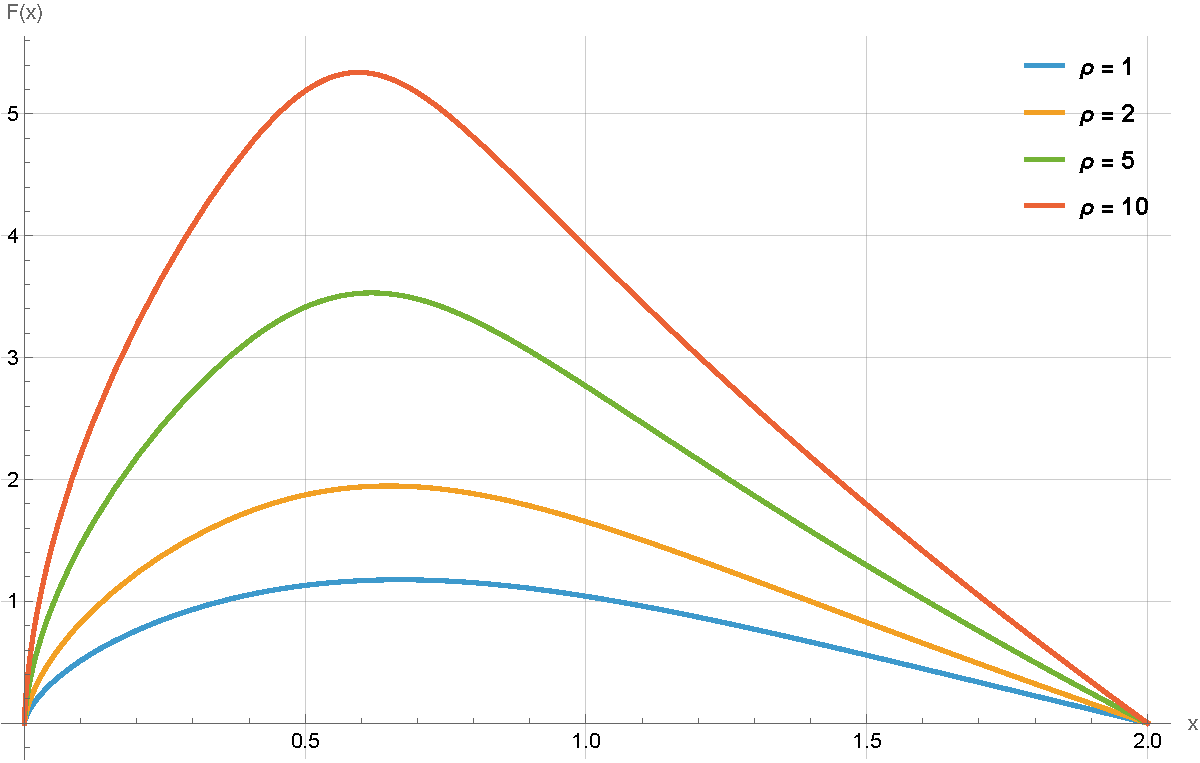
\includegraphics[width=\linewidth]{img/validation/P1/p1_R_value.pdf}
        \caption{P1 \textemdash~Fonction Valeur $F(x)$}\label{fig:RhoValueVisualisation1}
    \end{subfigure}
    \hfill
    \begin{subfigure}{0.45\linewidth}
        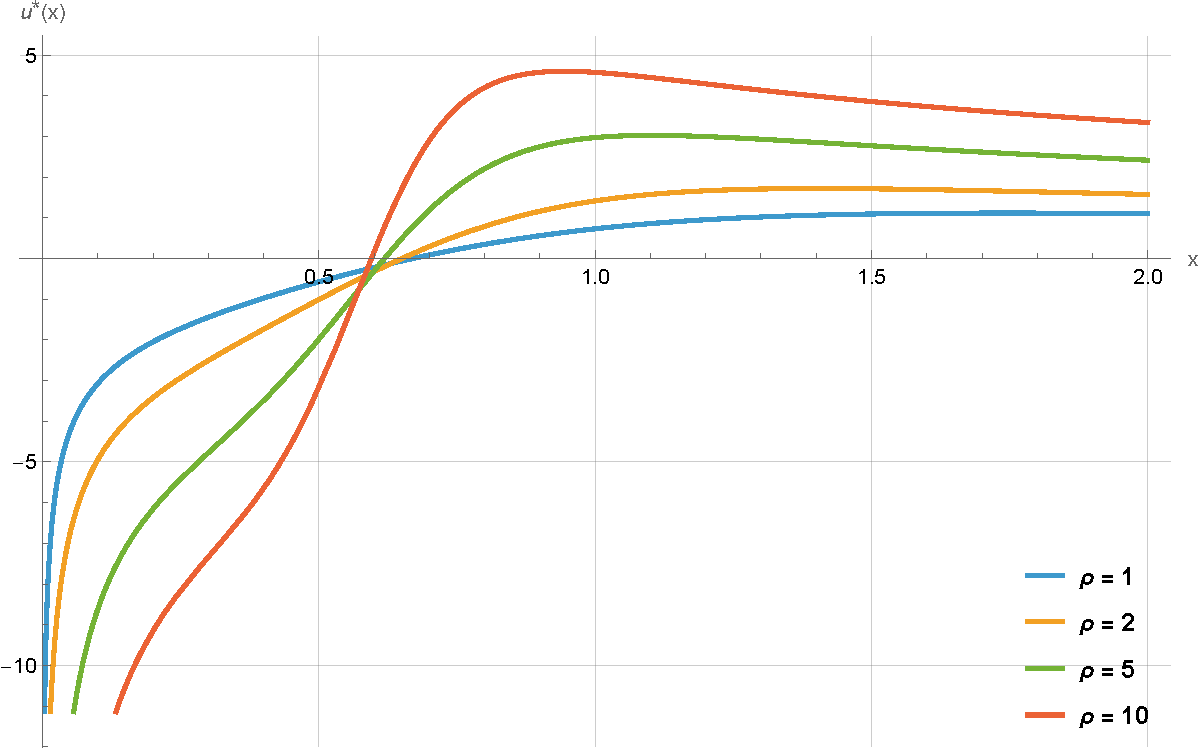
\includegraphics[width=\linewidth]{img/validation/P1/p1_R_control.pdf}
        \caption{P1 \textemdash~Contrôle Optimal $u^*(x)$}\label{fig:RhoControlVisualisation1}
    \end{subfigure}
    \caption{P1 \textemdash~Sensibilité du coût immédiat $r(x)=\rho$}\label{fig:RhoValueControlComparison1}
\end{figure}
\FloatBarrier\begin{figure}[htb]
    \centering
    \begin{subfigure}{0.45\linewidth}
        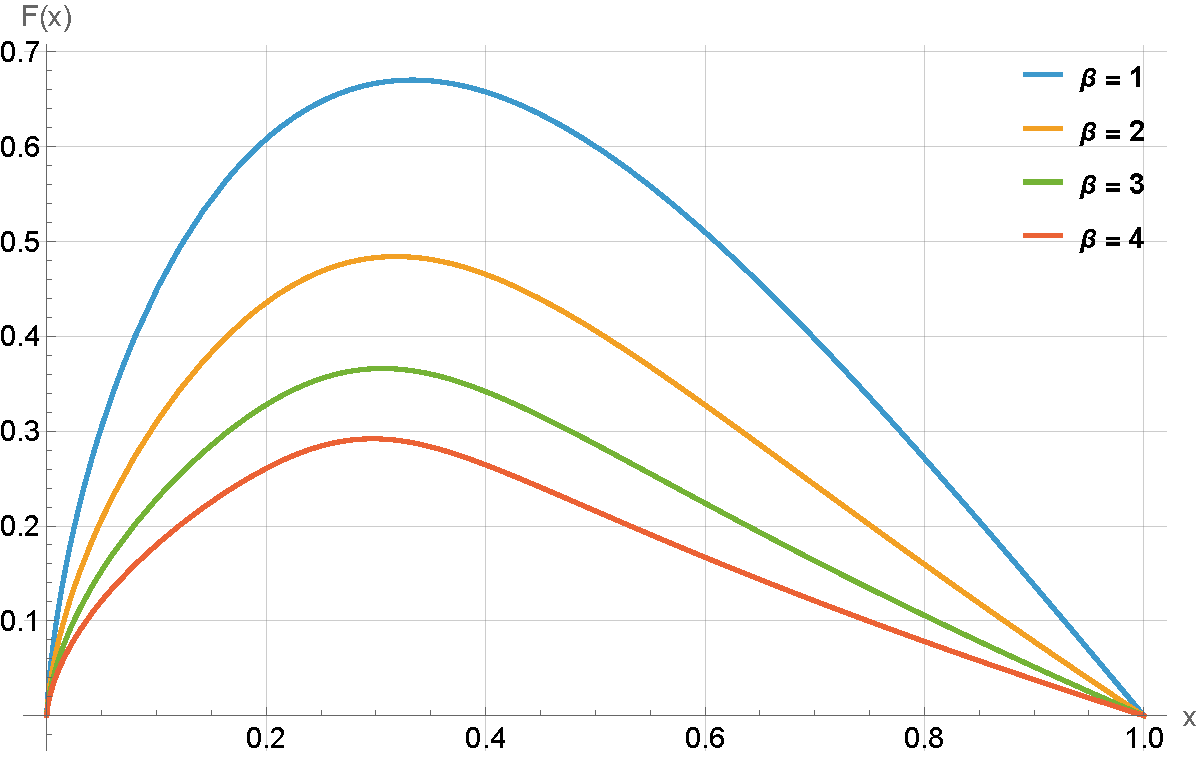
\includegraphics[width=\linewidth]{img/validation/P1/p1_B_value.pdf}
        \caption{P1 \textemdash~Fonction Valeur $F(x)$}\label{fig:BetaValueVisualisation1}
    \end{subfigure}
    \hfill
    \begin{subfigure}{0.45\linewidth}
        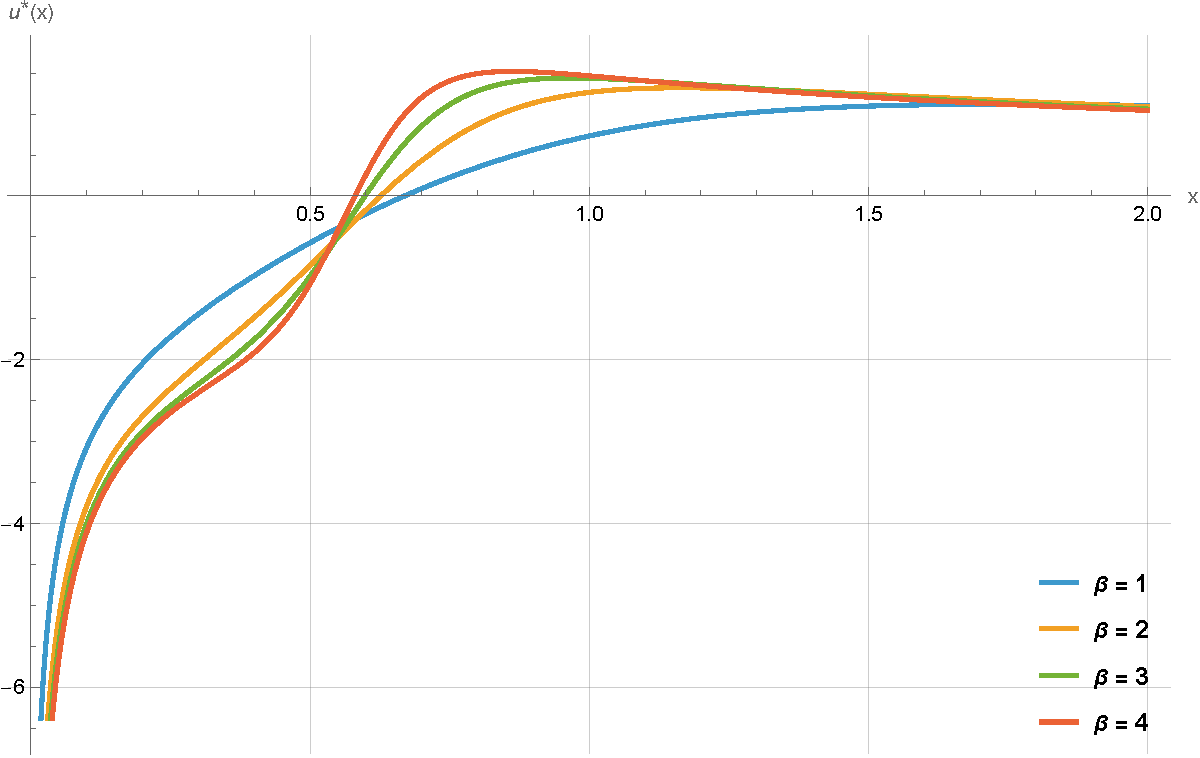
\includegraphics[width=\linewidth]{img/validation/P1/p1_B_control.pdf}
        \caption{P1 \textemdash~Contrôle Optimal $u^*(x)$}\label{fig:BetaControlVisualisation1}
    \end{subfigure}
    \caption{P1 \textemdash~Sensibilité du coût du contrôle $b(x)=\beta x$}\label{fig:BetaValueControlComparison}
\end{figure}
\FloatBarrier\begin{figure}[htb]
    \centering
    \begin{subfigure}{0.45\linewidth}
        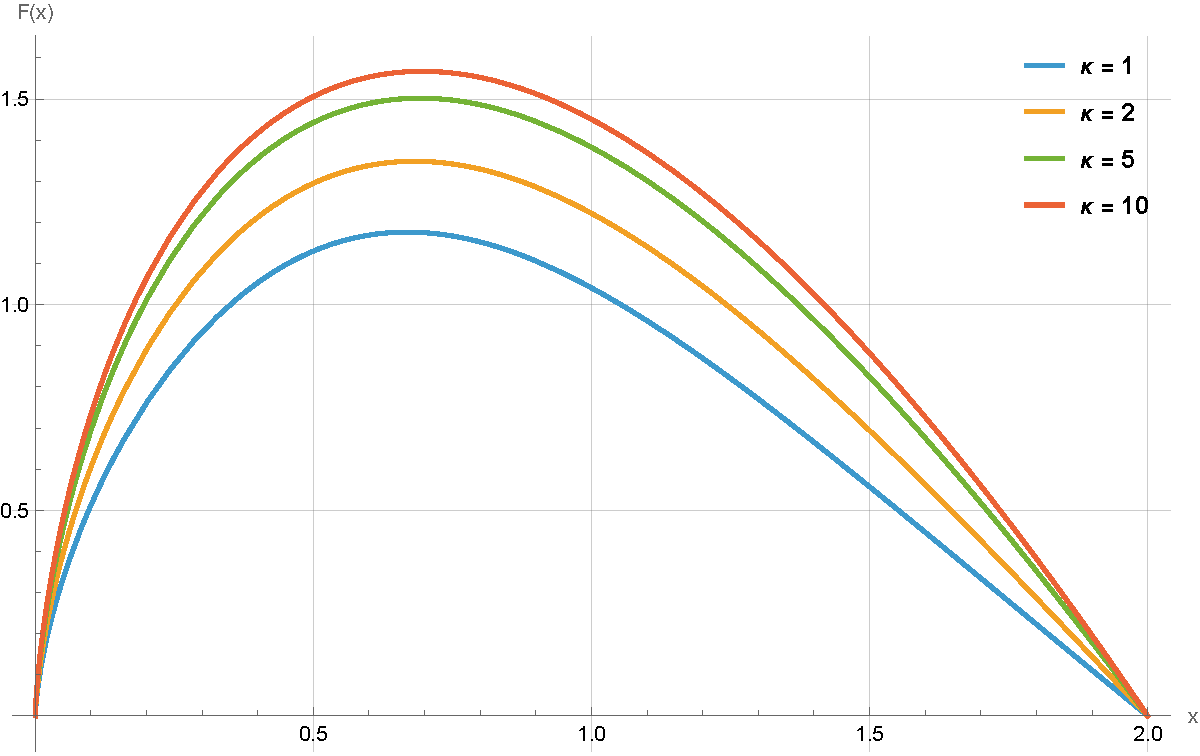
\includegraphics[width=\linewidth]{img/validation/P1/p1_K_value.pdf}
        \caption{P1 \textemdash~Fonction Valeur $F(x)$}\label{fig:KappaValueVisualisation1}
    \end{subfigure}
    \hfill
    \begin{subfigure}{0.45\linewidth}
        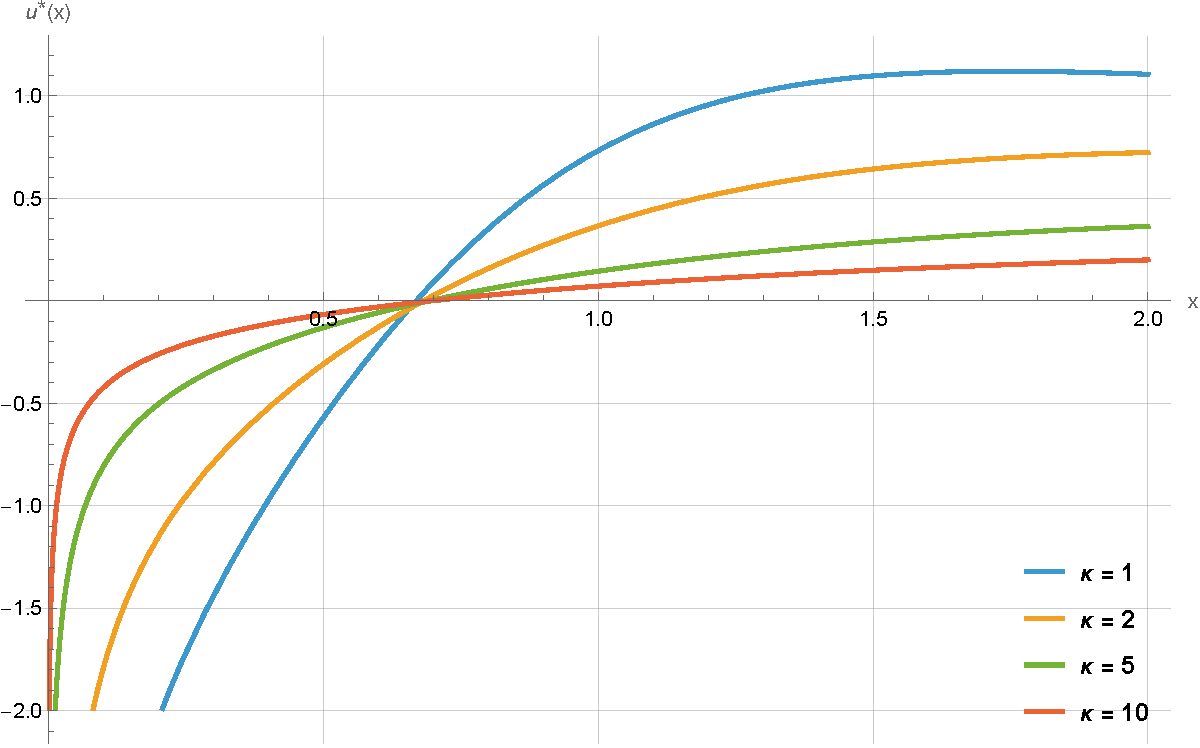
\includegraphics[width=\linewidth]{img/validation/P1/p1_K_control.pdf}
        \caption{P1 \textemdash~Contrôle Optimal $u^*(x)$}\label{fig:KappaControlVisualisation1}
    \end{subfigure}
    \caption{P1 \textemdash~Sensibilité de la pondération du contrôle $q(x)=\kappa x$}\label{fig:KappaValueControlComparison1}
\end{figure}
\FloatBarrier Une simulation d'une trajectoire contrôlée et d'une trajectoire non contrôlée est effectuée en utilisant un même tirage aléatoire, afin de permettre une comparaison pertinente entre les deux dynamiques. Les paramètres du processus \acs{CIR} sont ceux introduits en début de section, avec $\rho = \beta = \kappa = 1$.
\begin{figure}[htb]
    \centering
    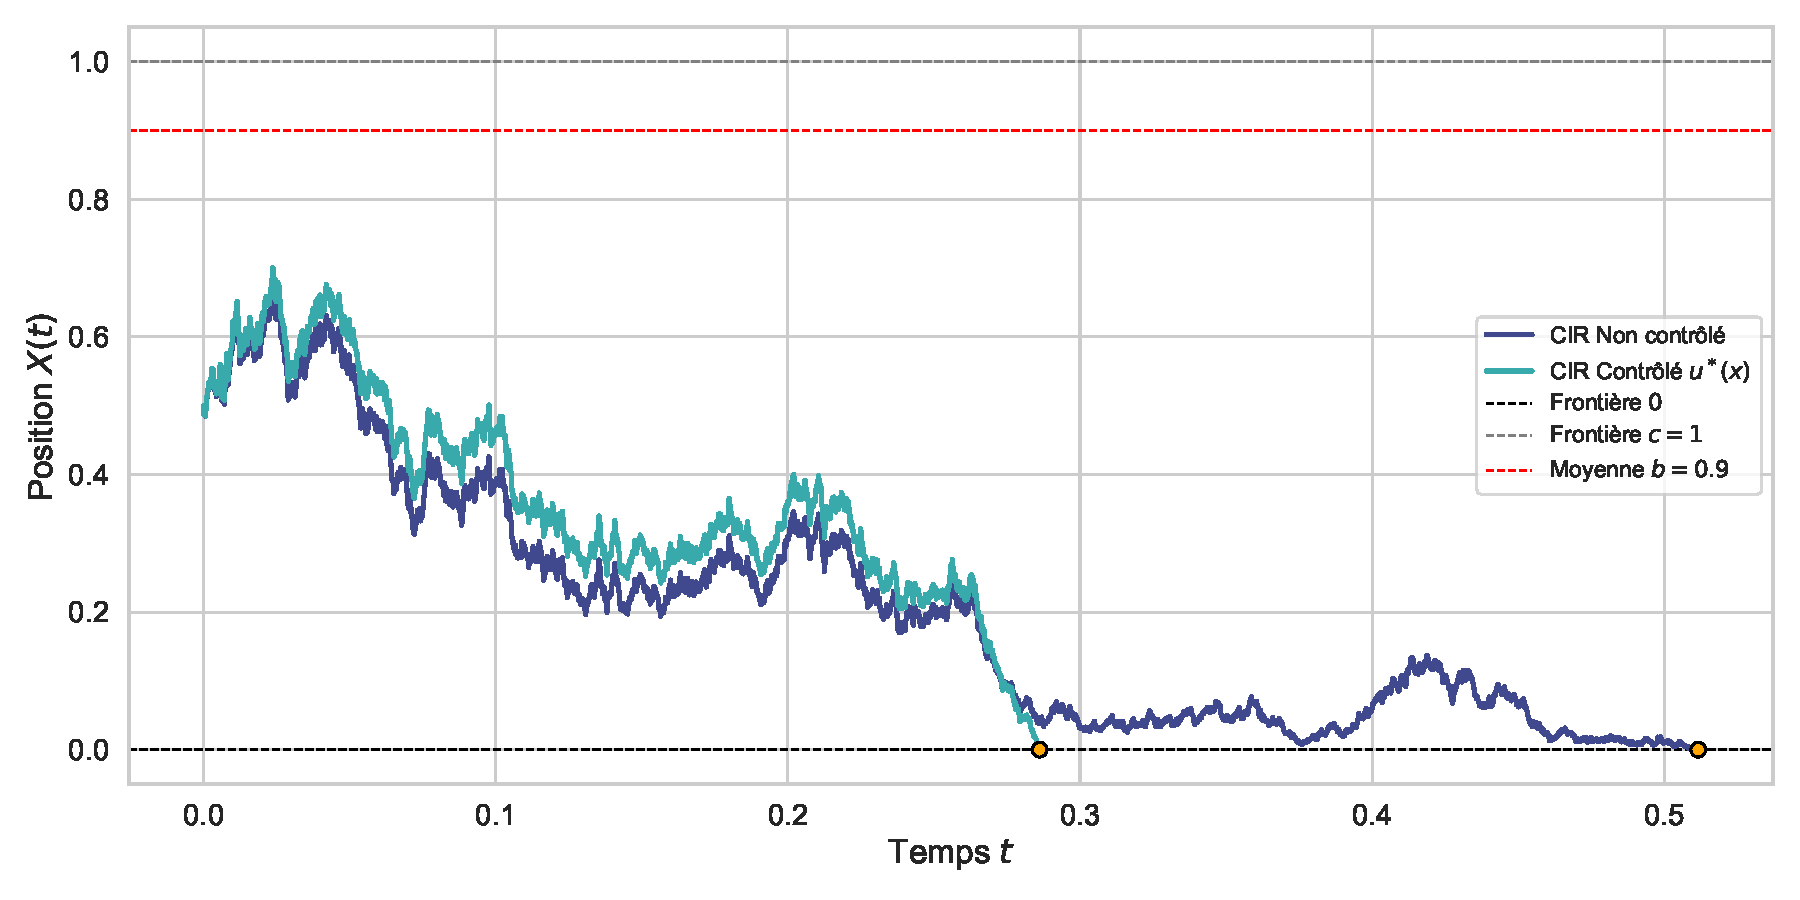
\includegraphics[width=0.9\linewidth]{img/validation/P1/p1_control_simulation.pdf}
    \caption{P1 \textemdash~Visualisation de l'effet de la commande optimale}
\end{figure}
\FloatBarrier\subsubsection{Problème linéarisable 2 \textemdash~P2}\phantom{}\\
Les résultats du problème (\ref{p2}) sont analysés. D'un côté, les fonctions $r(x)$, $b(x)$ et $q(x)$ sont définies en (\ref{p2}). D'un autre côté, la fonction valeur $F(x)$ est définie par (\ref{sol_control_2},~\ref{control_constants}) et le contrôle optimal est défini par (\ref{optimal_control_2}). Dans un premier temps, les coûts sont fixés: $\rho=\beta=\kappa=1$.
\begin{figure}[htb]
    \centering
    \begin{subfigure}{0.45\linewidth}
        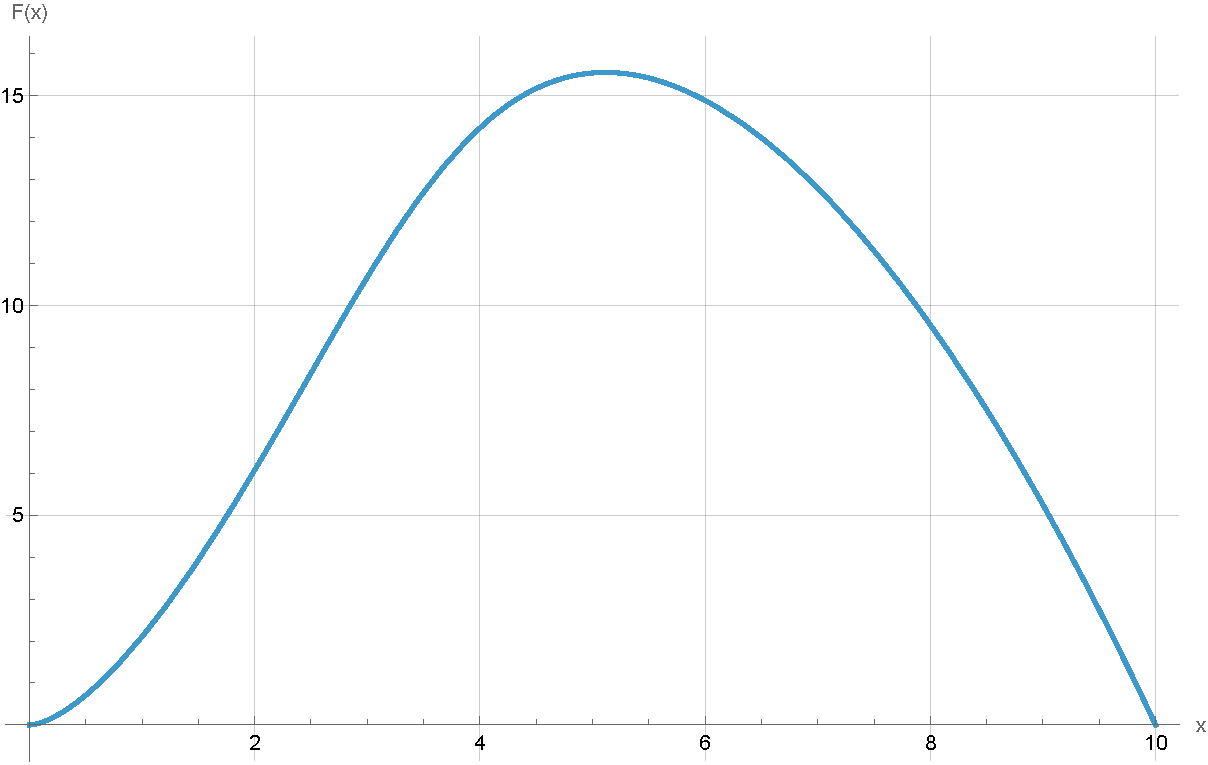
\includegraphics[width=\linewidth]{img/validation/P2/p2_value.pdf}
        \caption{P2 \textemdash~Fonction Valeur $F(x)$}\label{fig:ValueVisualisation2}
    \end{subfigure}
    \hfill
    \begin{subfigure}{0.45\linewidth}
        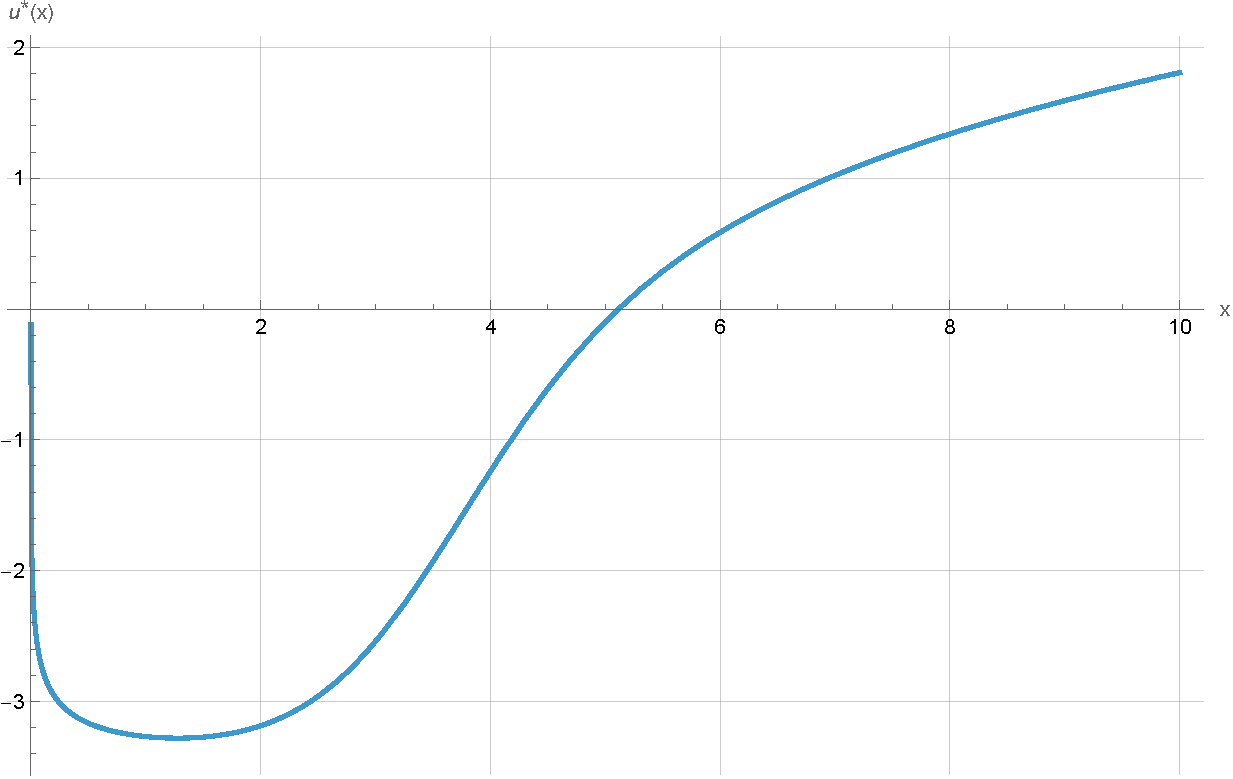
\includegraphics[width=\linewidth]{img/validation/P2/p2_control.pdf}
        \caption{P2 \textemdash~Contrôle Optimal $u^*(x)$}\label{fig:ControlVisualisation2}
    \end{subfigure}
    \caption{P2 \textemdash~Visualisation de la fonction valeur et du contrôle optimal}\label{fig:ValueControlComparison2}
\end{figure}\FloatBarrier Dans un second temps, et comme ce qui précède, la sensibilité des coûts est analysée, en fonction des mêmes valeurs paramètres $\rho$, $\beta$ et $\kappa$.
\begin{figure}[htb]
    \centering
    \begin{subfigure}{0.45\linewidth}
        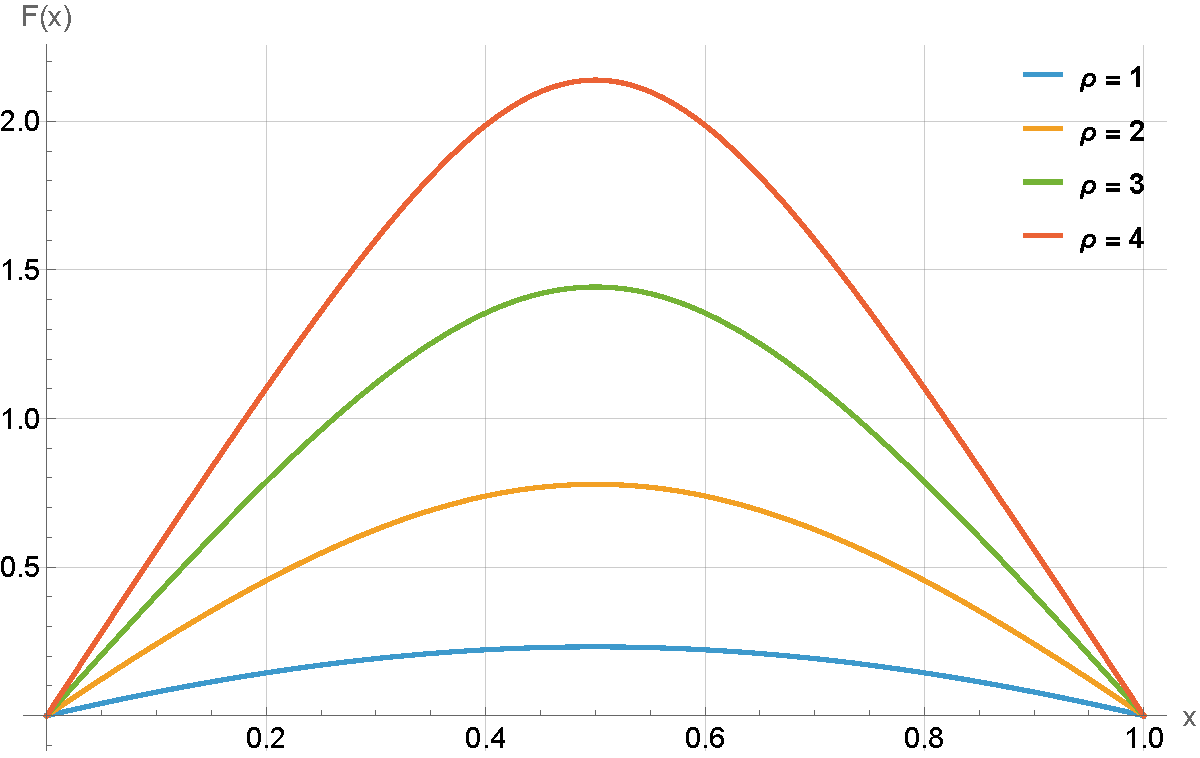
\includegraphics[width=\linewidth]{img/validation/P2/p2_R_value.pdf}
        \caption{P2 \textemdash~Fonction Valeur $F(x)$}\label{fig:RhoValueVisualisation2}
    \end{subfigure}
    \hfill
    \begin{subfigure}{0.45\linewidth}
        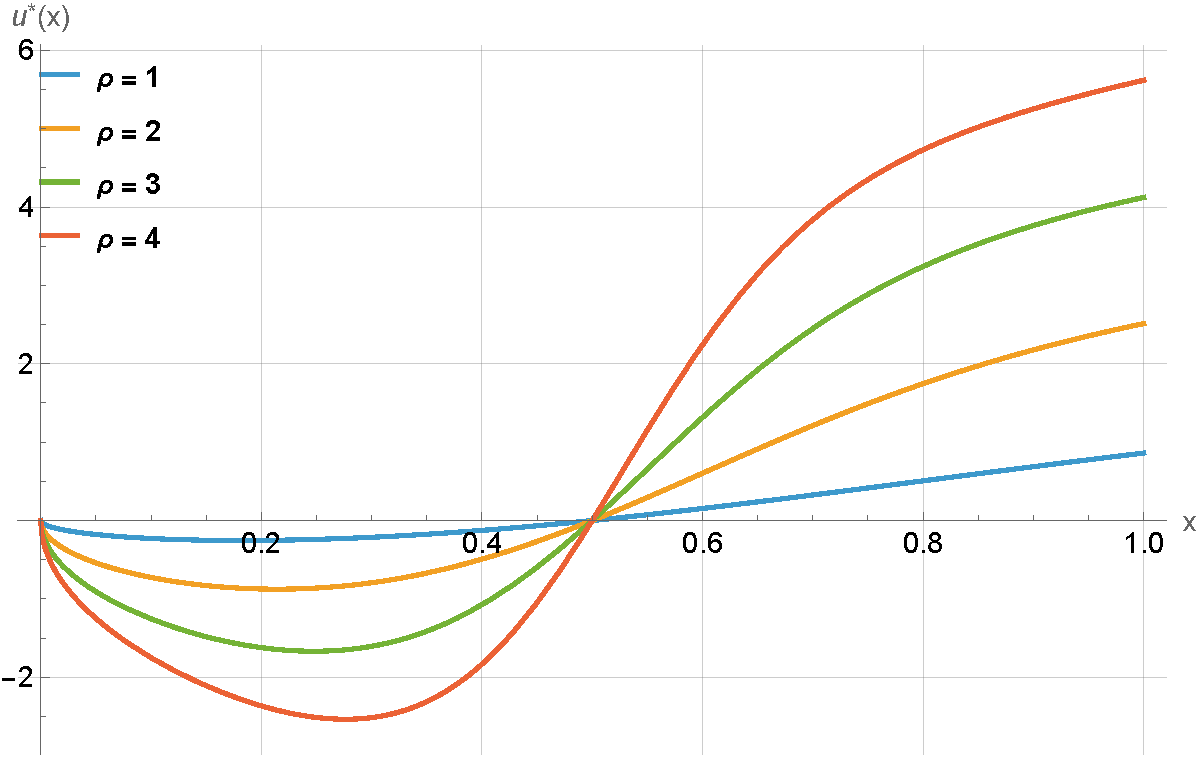
\includegraphics[width=\linewidth]{img/validation/P2/p2_R_control.pdf}
        \caption{P2 \textemdash~Contrôle Optimal $u^*(x)$}\label{fig:RhoControlVisualisation2}
    \end{subfigure}
    \caption{P2 \textemdash~Sensibilité du coût immédiat $r(x)=\rho x$}\label{fig:RhoValueControlComparison2}
\end{figure}
\FloatBarrier\begin{figure}[htb]
    \centering
    \begin{subfigure}{0.45\linewidth}
        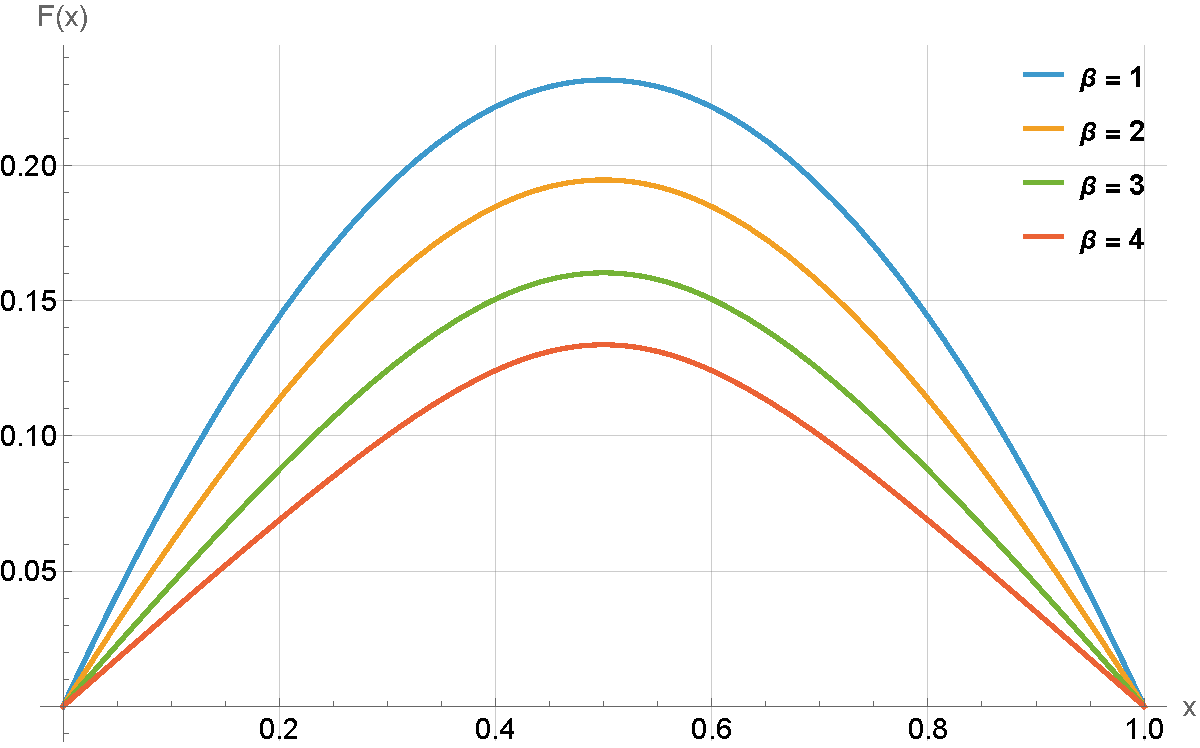
\includegraphics[width=\linewidth]{img/validation/P2/p2_B_value.pdf}
        \caption{P2 \textemdash~Fonction Valeur $F(x)$}\label{fig:BetaValueVisualisation2}
    \end{subfigure}
    \hfill
    \begin{subfigure}{0.45\linewidth}
        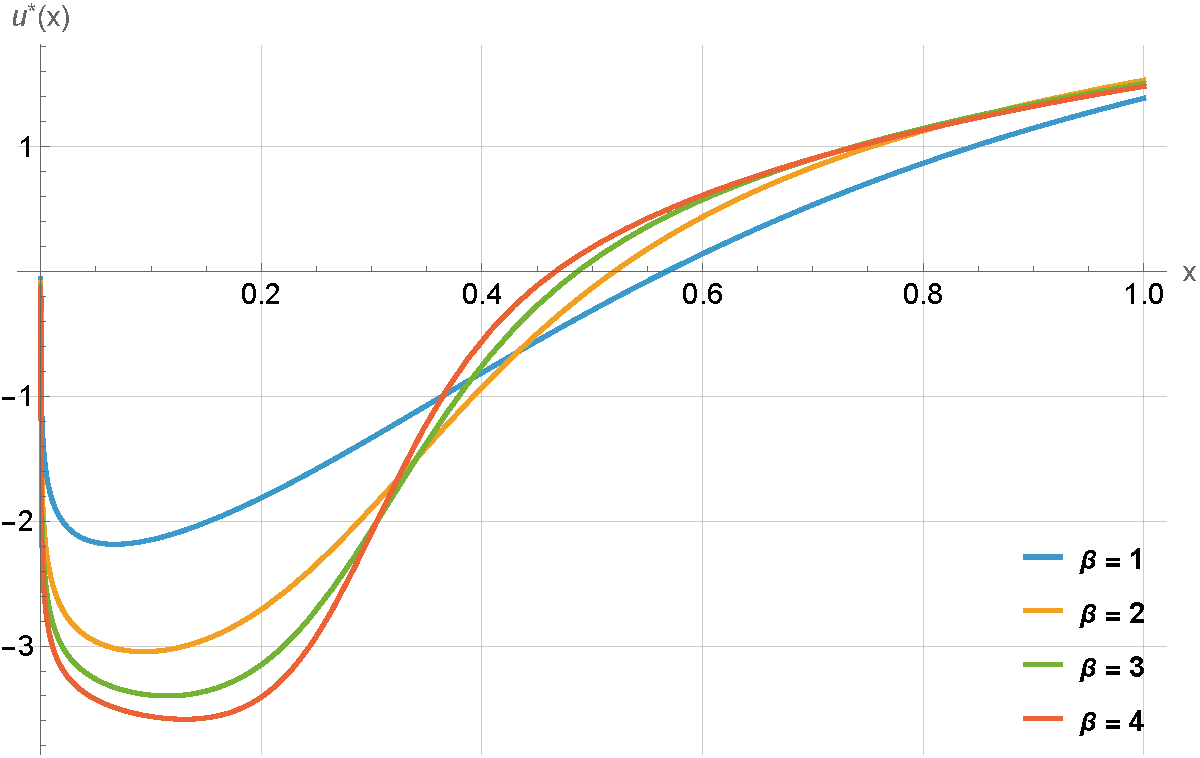
\includegraphics[width=\linewidth]{img/validation/P2/p2_B_control.pdf}
        \caption{P2 \textemdash~Contrôle Optimal $u^*(x)$}\label{fig:BetaControlVisualisation2}
    \end{subfigure}
    \caption{P2 \textemdash~Sensibilité du coût du contrôle $b(x)=\beta \sqrt{x}$}\label{fig:BetaValueControlComparison1}
\end{figure}
\FloatBarrier\begin{figure}[htb]
    \centering
    \begin{subfigure}{0.45\linewidth}
        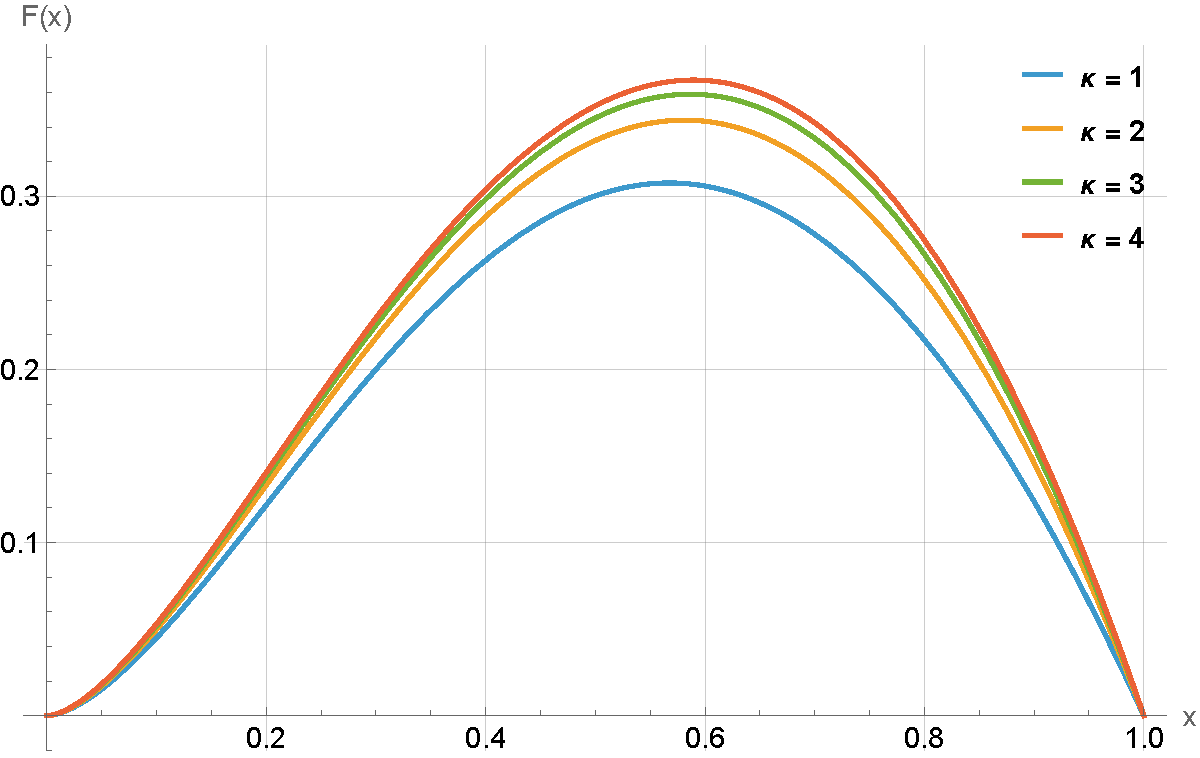
\includegraphics[width=\linewidth]{img/validation/P2/p2_K_value.pdf}
        \caption{P2 \textemdash~Fonction Valeur $F(x)$}\label{fig:KappaValueVisualisation2}
    \end{subfigure}
    \hfill
    \begin{subfigure}{0.45\linewidth}
        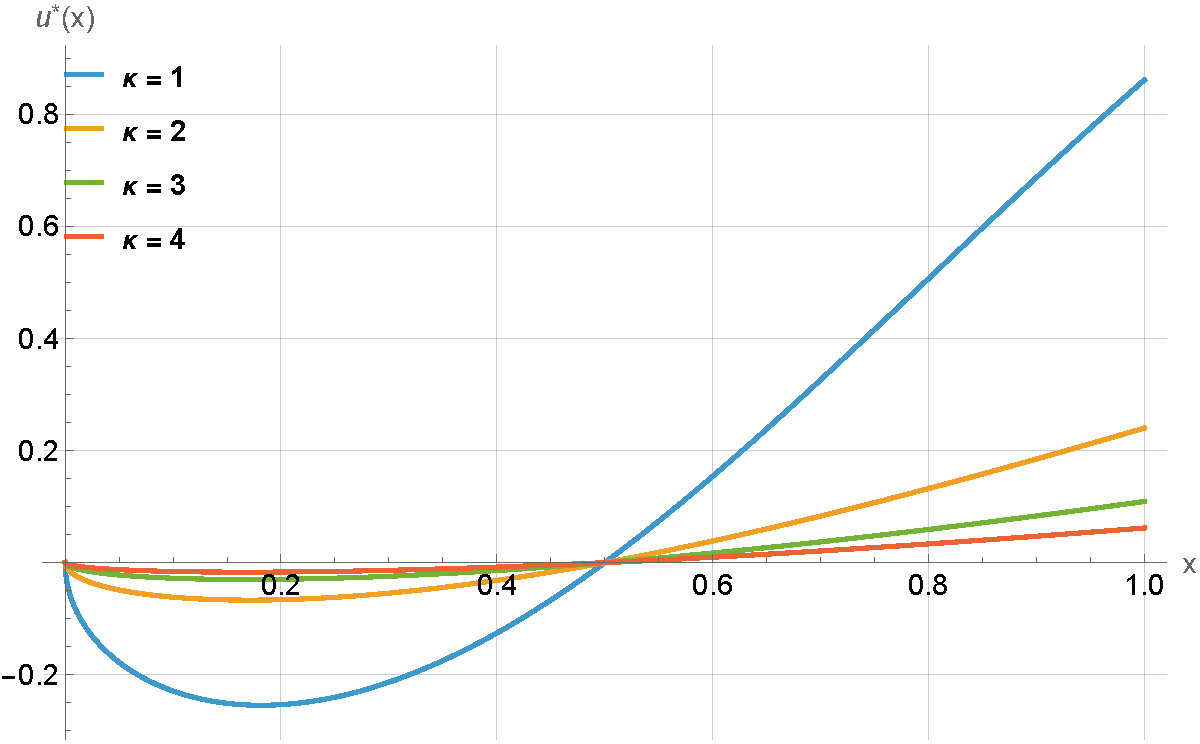
\includegraphics[width=\linewidth]{img/validation/P2/p2_K_control.pdf}
        \caption{P2 \textemdash~Contrôle Optimal $u^*(x)$}\label{fig:KappaControlVisualisation2}
    \end{subfigure}
    \caption{P2 \textemdash~Sensibilité de la pondération du contrôle $q(x)=\kappa x$}\label{fig:KappaValueControlComparison2}
\end{figure}
\FloatBarrier Comme précédemment, une trajectoire contrôlée est comparée à une trajectoire non contrôlée à partir d'un même tirage aléatoire. Les paramètres utilisés sont identiques à ceux de la dernière simulation.
\begin{figure}[htb]
    \centering
    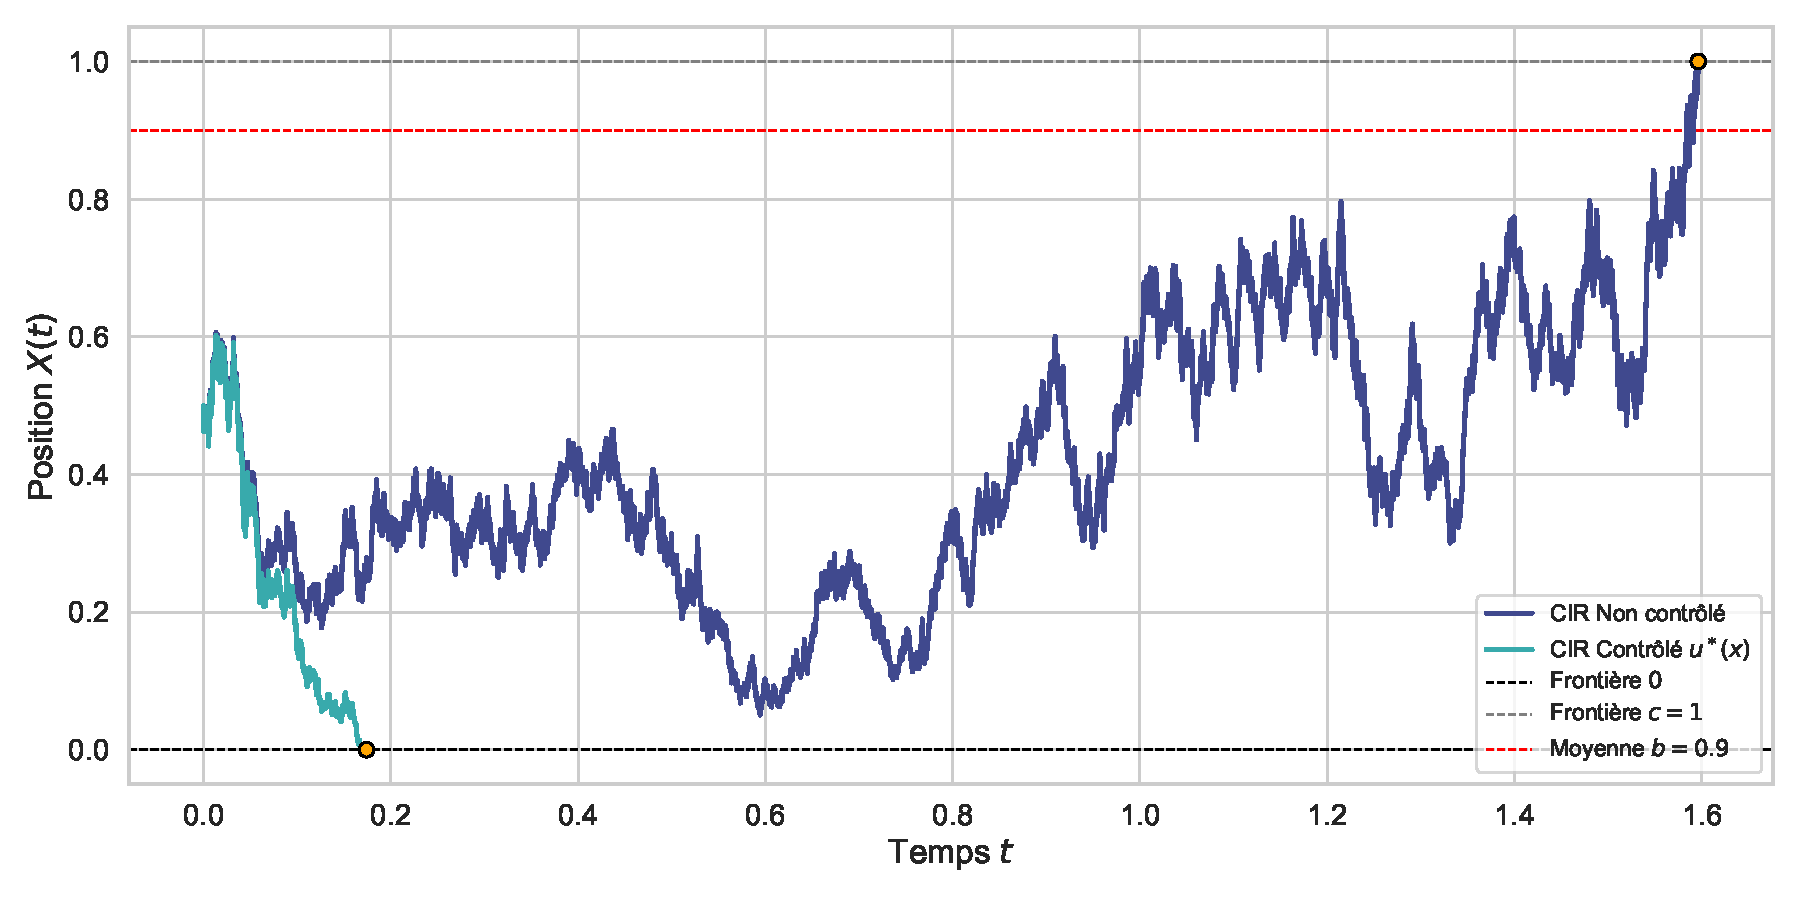
\includegraphics[width=0.9\linewidth]{img/validation/P2/p2_control_simulation.pdf}
    \caption{P2 \textemdash~Visualisation de l'effet de la commande optimale}
\end{figure}
\subsubsection{Problème non linéarisable \textemdash~P3}\phantom{}\\
Le problème (\ref{p3}) est porté à l'étude. L'expression de la fonction valeur (\ref{sol_control_3}) ainsi que la commande optimale (\ref{optimal_control_3}) sont tracés.
\begin{figure}[htb]
    \centering
    \begin{subfigure}{0.45\linewidth}
        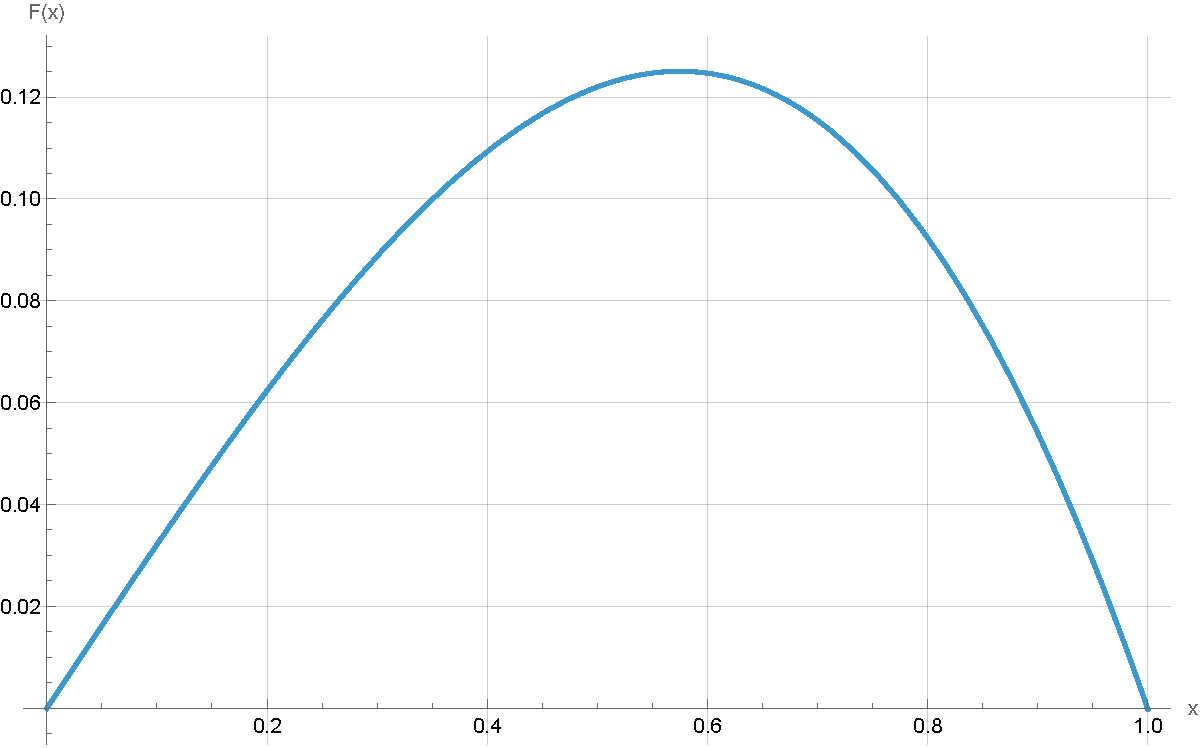
\includegraphics[width=\linewidth]{img/validation/P3/p3_value.pdf}
        \caption{P3 \textemdash~Fonction Valeur $F(x)$}\label{fig:ValueVisualisation3}
    \end{subfigure}
    \hfill
    \begin{subfigure}{0.45\linewidth}
        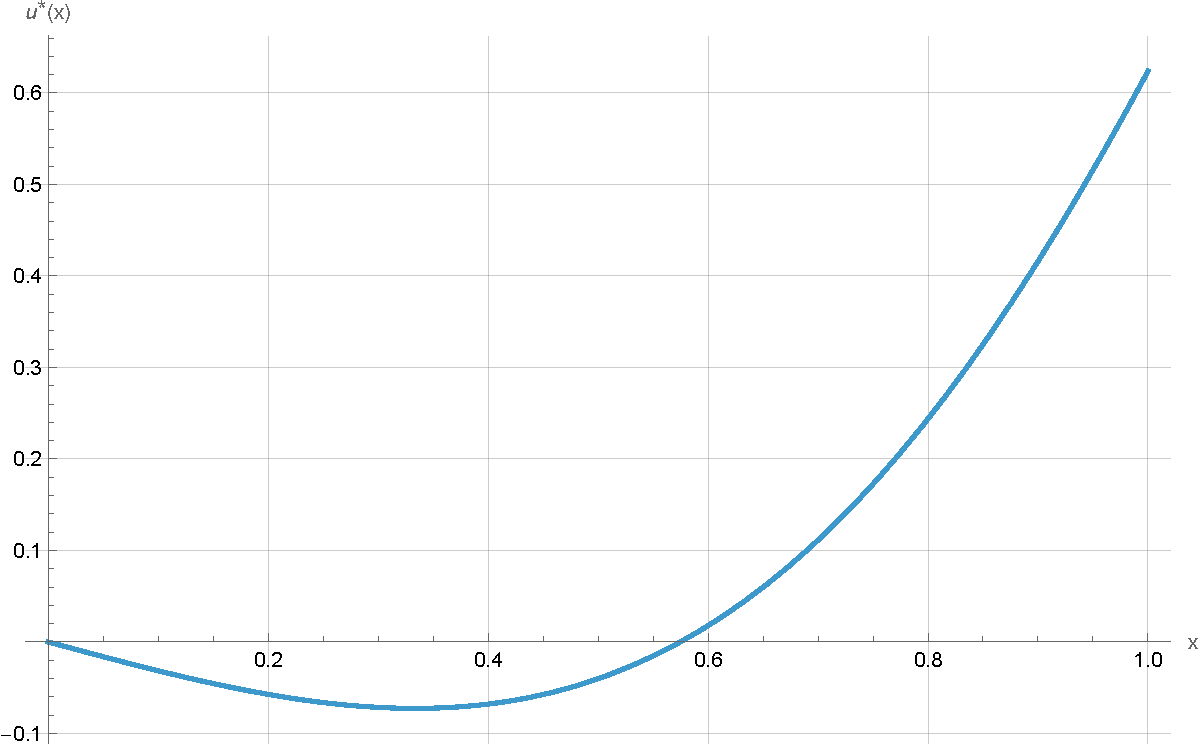
\includegraphics[width=\linewidth]{img/validation/P3/p3_control.pdf}
        \caption{P3 \textemdash~Contrôle Optimal $u^*(x)$}\label{fig:ControlVisualisation3}
    \end{subfigure}
    \caption{P3 \textemdash~Visualisation de la fonction valeur et du contrôle optimal}\label{fig:ValueControlComparison3}
\end{figure}
\FloatBarrier Toujours dans la même optique de visualisation de l'effet du contrôle, une simulation est effectuée. 
\begin{figure}[htb]
    \centering
    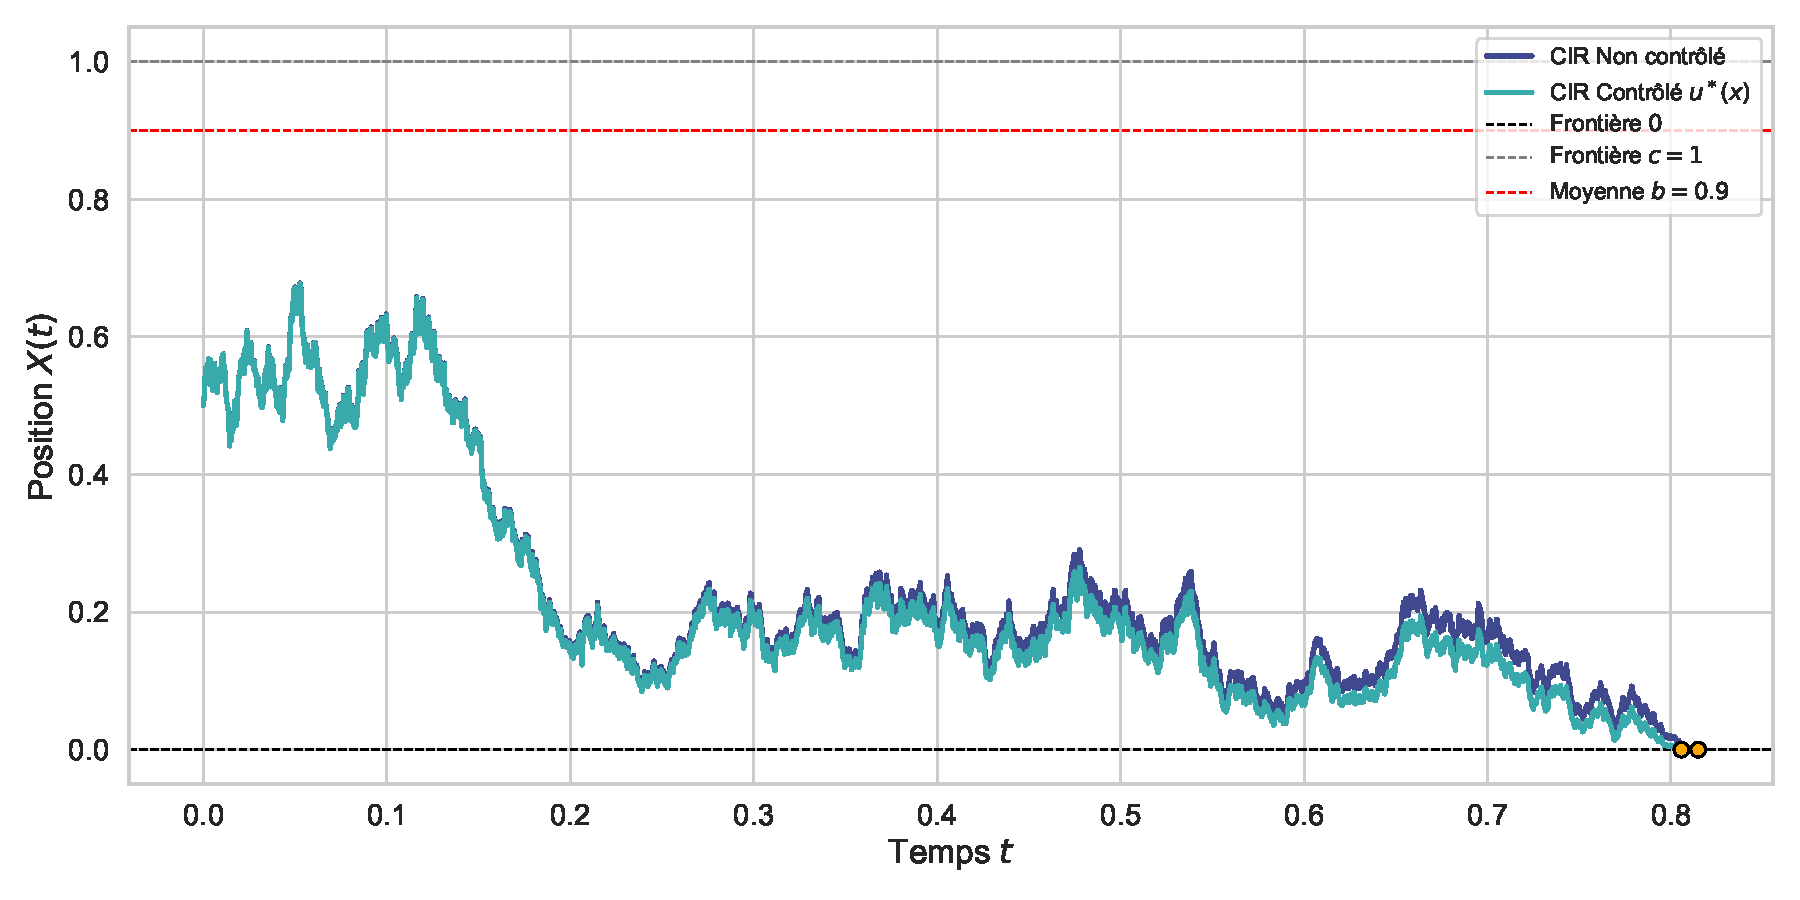
\includegraphics[width=0.9\linewidth]{img/validation/P3/p3_control_simulation.pdf}
    \caption{P3 \textemdash~Visualisation de l'effet de la commande optimale}\label{fig:Simulation3}
\end{figure}
\paragraph{Analyse}\phantom{}\\
Il est important de souligner que, dans les trois problèmes étudiés et pour les différentes valeurs des paramètres considérés:
\begin{itemize}
    \item Les conditions aux limites $F(0)=F(c)=0$ sont toujours respectées;
    \item La fonction valeur est toujours positive, le coût encouru étant nécessairement positif;
    \item Le contrôle optimal est généralement négatif sur \( x \in \left(0, \frac{c}{2}\right) \), l'optimiseur cherchant à diriger rapidement le processus vers la frontière \( 0 \), plus proche. Inversement, pour \( x \in \left(\frac{c}{2}, c\right) \), le contrôle devient positif afin d'accélérer l'atteinte de la frontière supérieure \( c \);
    \item Une augmentation du coût immédiat $\rho$, induisant une hausse du coût encouru, entraîne un renforcement du contrôle optimal ($|u^*(x)|$ augmente), traduisant ainsi une volonté accrue de quitter l'intervalle aussi rapidement que possible;
    \item Une hausse du coût du contrôle $\beta$ incite à intensifier le contrôle optimal afin de quitter l'intervalle plus rapidement. Cette stratégie réduit la durée d'exposition au coût instantané, ce qui compense partiellement le surcoût du contrôle et diminue le coût total encouru $F(x)$;
    \item Une augmentation du poids pénalisant le contrôle $\kappa$, induisant une hausse du coût encouru, entraîne une relaxation du contrôle optimal. En effet, plus le poids du contrôle est élevé, moins il est intéressant d'appliquer un contrôle fort;
    \item Les simulations mettent en évidence l'effet du contrôle optimal, qui accélère la sortie du processus par rapport au cas non contrôlé. Pour valider cette observation, 1000 trajectoires sont simulées pour chaque problème, et la durée moyenne jusqu'à la sortie est comparée. Un facteur d'accélération est ensuite estimé:
    \begin{table}[htb]
        \centering
        \caption{Accélérations moyennes du temps de sortie}\label{tab:acceleration_results}
        \renewcommand{\arraystretch}{1.1}
        \begin{tabular}{||c|c||}
        \hline
        Problème & Accélération Moyenne \\\hline\hline
        P1 & 2.660552 \\
        P2 & 2.690582 \\
        P3 & 1.065163 \\\hline
        \end{tabular}
    \end{table}\FloatBarrier Voir annexe~\ref{control_simulations} pour les détails du calcul; 
    \item La suppression du retour à la moyenne entraîne une réduction de l'intensité du contrôle (voir~\ref{fig:ControlVisualisation3},~\ref{fig:Simulation3}). En l'absence de force de rappel, le processus est naturellement plus enclin à atteindre une des deux frontières, ce qui permet d'intervenir avec une commande de faible amplitude.
\end{itemize}
Ainsi, les expressions obtenues pour la fonction valeur $F(x)$ et le contrôle optimal $u^*(x)$ sont validées.
\paragraph{Politiques Optimales}\phantom{}\\
En effectuant plusieurs simulations et en analysant les représentations des différentes commandes $u^*(x)$ obtenues (\ref{fig:ControlVisualisation1},~\ref{fig:ControlVisualisation2},~\ref{fig:ControlVisualisation3}), il est possible de caractériser les différentes stratégies optimales dans le cadre de chaque problème étudié:
\begin{itemize}
    \item \textbf{Stratégie P1 \textemdash~Modulation Adaptative}\\
    La stratégie optimale consiste à moduler l'intensité du contrôle selon la position. L'optimiseur suit la dynamique naturelle du processus: il accompagne les tendances favorables avec un contrôle modéré, puis intervient davantage à l'approche d'une frontière. Lors d'un retournement de tendance, il retarde volontairement sa réponse, espérant une reprise favorable dans la direction initiale. Ce comportement vise à limiter les coûts de contrôle (\( b(x) = x \), \( q(x) = x \)) tout en assurant la sortie. Globalement, la stratégie cherche un compromis entre passivité opportuniste et action ciblée selon la position et la tendance du processus.

    \item \textbf{Stratégie P2 \textemdash~Attente et Attaque}\\
    La stratégie commence par une phase d'observation sans intervention, les trajectoires contrôlée et non contrôlée se superposant au départ. Lorsqu'une tendance claire apparaît, le contrôle devient rapidement agressif pour provoquer la sortie. Contrairement au cas P1, l'optimiseur n'attend pas en cas d'inversion de tendance mais intensifie son contrôle. Les sorties s'effectuent souvent par le bas, ce qui est cohérent avec les coûts faibles dans cette zone (\( r(x) = x \), \( b(x) = \sqrt{x} \), \( q(x) = x \)). Il s'agit d'une stratégie opportuniste suivie d'une action déterminée.

    \item \textbf{Stratégie P3 \textemdash~Évasion Passive}\\
    Le contrôle est minimal et les trajectoires restent proches du non contrôlé. L'évasion se produit juste avant celle du processus non contrôlé, ce qui traduit une stratégie très passive. Le contrôle n'est appliqué que lorsqu'il devient strictement nécessaire, sans forcer la dynamique. Cette approche s'explique par les coûts élevés liés aux grandes valeurs de \( x \) (\( r(x) = x^2 \), \( b(x) = x \)), et l'absence d'incitation à intervenir fortement (\( q(x) \equiv 1 \)). L'optimiseur attend que la dynamique seule suffise à atteindre la frontière.
\end{itemize}
\section{Diffusion avec sauts}
Cette section est consacrée à la présentation des résultats portants sur le \acs{CIR} avec sauts défini en (\ref{jump_cir_sde}).
\subsection{Fonction Temps moyen \textemdash~Sauts uniformes}
Les paramètres utilisés sont ceux introduits lors de l'étude du temps moyen de sortie, à la sous-partie (\ref{subsection_mean_jumps}). Les fonctions \( m(x) \) (avec sauts) et \( m_0(x) \) (sans sauts), données respectivement par (\ref{sol_mean_with_jumps}) et (\ref{sol_mean_with_0_jumps}), sont tracées.
\paragraph{Visualisation}\phantom{}
\begin{figure}[htb]
    \centering
    \begin{subfigure}{0.45\linewidth}
        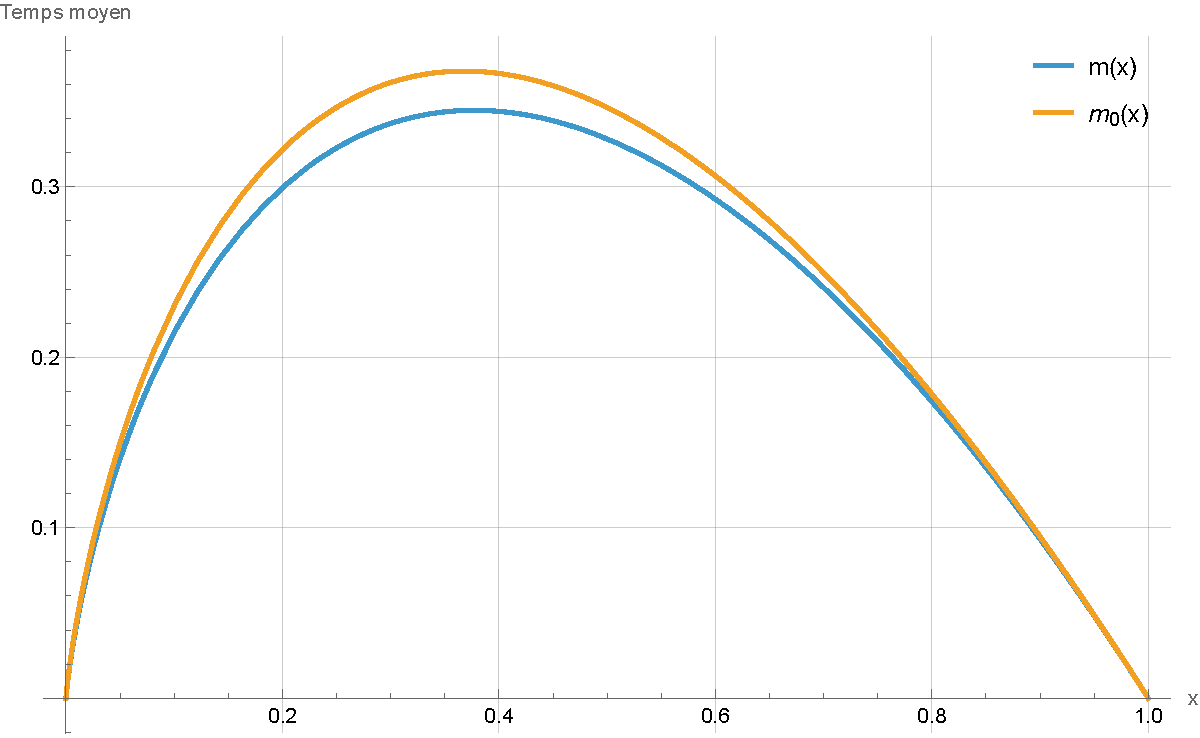
\includegraphics[width=\linewidth]{img/validation/Jumps/mean_jumps.pdf}
        \caption{Fréquence des sauts $\lambda=1$}
    \end{subfigure}
    \hfill
    \begin{subfigure}{0.45\linewidth}
        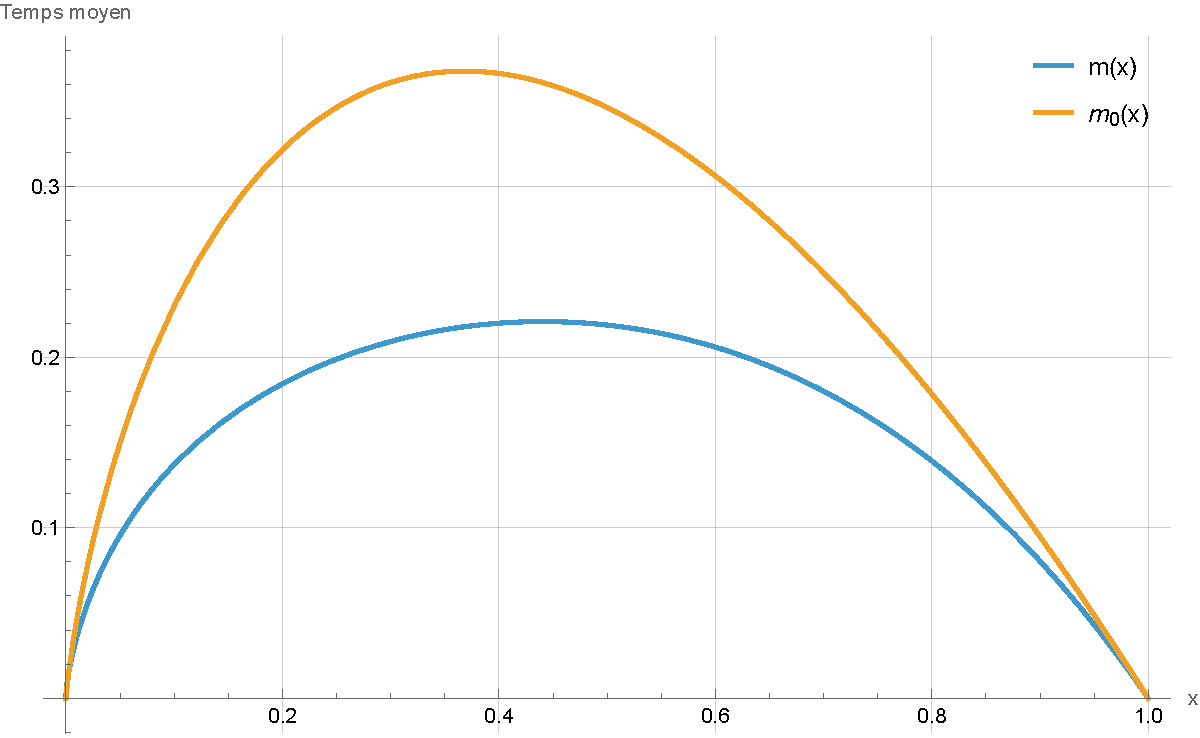
\includegraphics[width=\linewidth]{img/validation/Jumps/mean_big_jumps.pdf}
        \caption{Fréquence des sauts $\lambda=10$}
    \end{subfigure}
    \caption{Visualisation des temps moyens de sortie $m(x)$ et $m_0(x)$}\label{fig:JumpsMeanVisualisation}
\end{figure}
\FloatBarrier\paragraph{Analyse}\phantom{}\\
Il convient de souligner les observations suivantes:
\begin{itemize}
    \item Les conditions aux limites \( m(0) = m(c) = m_0(0) = m_0(c) = 0 \) sont bien vérifiées.
    \item Le temps moyen de sortie en présence de sauts ($m(x)$ en bleu) est inférieur à celui observé sans sauts ($m_0(x)$ en orange), ce qui illustre l'accélération du processus induite par ces derniers.
    \item Une augmentation de la fréquence des sauts $\lambda$ induit une diminution du temps moyen de sortie. Ce comportement est attendu comme les sauts augmente la probabilité que le \acs{CIR} quitte l'intervalle rapidement.
\end{itemize}

\subsection{Fonction Probabilité de sortie en zéro \textemdash~Sauts uniformes}
Les paramètres considérés sont ceux définis dans l'étude de la probabilité de sortie en zéro, présentée en sous-partie (\ref{subsection_probability_jumps}). Les fonctions \( p(x) \) (avec sauts) et \( p_0(x) \) (sans sauts), correspondant respectivement aux expressions (\ref{sol_probability_with_jumps}) et (\ref{sol_probability}), sont représentées graphiquement.
\paragraph{Visualisation}\phantom{}
\begin{figure}[htb]
    \centering
    \begin{subfigure}{0.45\linewidth}
        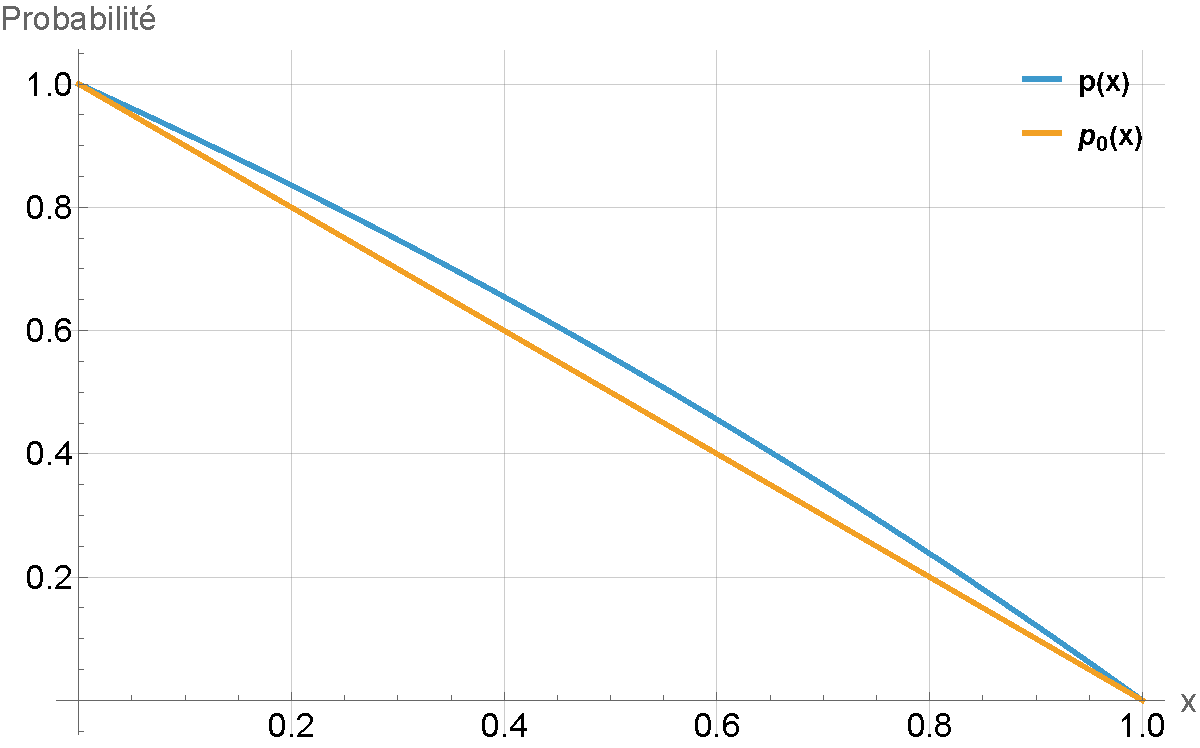
\includegraphics[width=\linewidth]{img/validation/Jumps/probability_jumps.pdf}
        \caption{Fréquence des sauts $\lambda=1$}
    \end{subfigure}
    \hfill
    \begin{subfigure}{0.45\linewidth}
        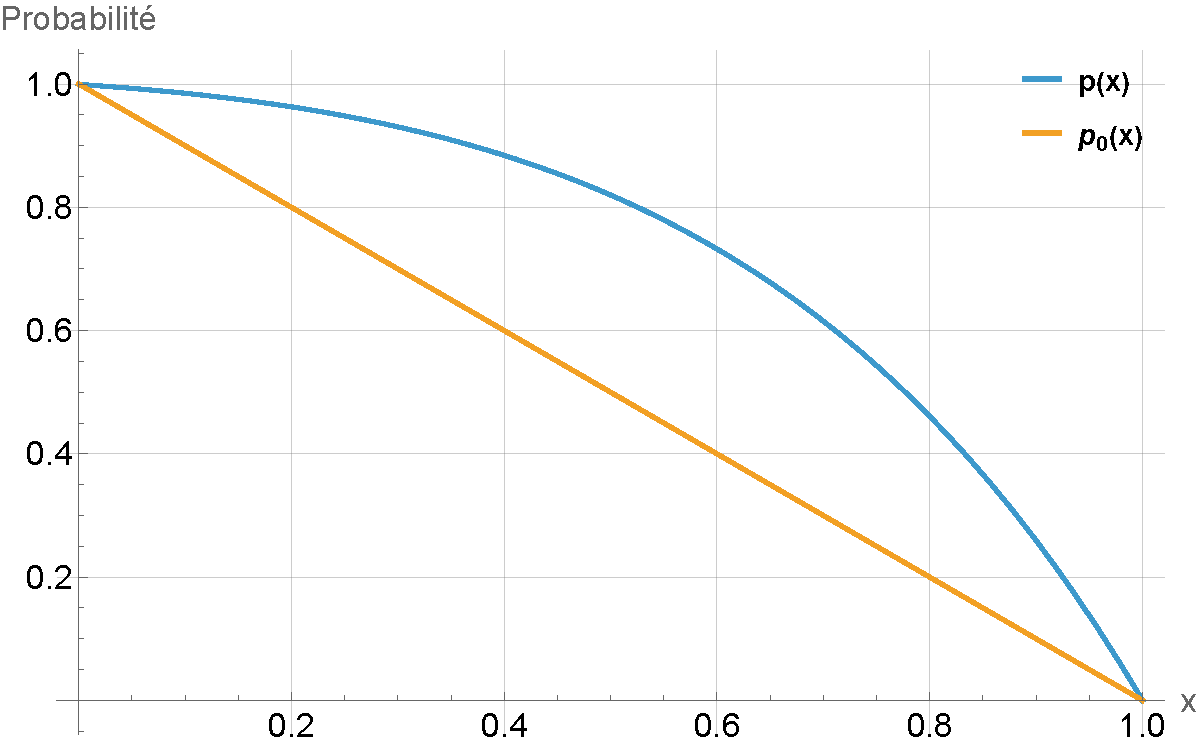
\includegraphics[width=\linewidth]{img/validation/Jumps/probability_big_jumps.pdf}
        \caption{Fréquence des sauts $\lambda=10$}
    \end{subfigure}
    \caption{Visualisation des probabilités de sortir en zéro $p(x)$ et $p_0(x)$}\label{fig:JumpsProbabilityVisualisation}
\end{figure}
\FloatBarrier\paragraph{Analyse}\mbox{}\\
Les observations suivantes peuvent être formulées:
\begin{itemize}
    \item Les conditions aux limites sont correctement satisfaites, à savoir \( p(0) = p_0(0) = 1 \) et \( p(c) = p_0(c) = 0 \).
    \item Les sauts étant négatifs, ils favorisent une sortie par la borne inférieure. La probabilité de franchissement par zéro est donc plus élevée dans le cas avec sauts ($p(x)$ en bleu);
    \item Une augmentation de la fréquence des sauts $\lambda$ entraîne une augmentation considérable de la probabilité de sortir par zéro. En effet, les sauts étant négatifs, leur multiplication tend à entraîner le processus vers la borne inférieure.
\end{itemize}

\subsection{Fonction Dépassement Moyen \textemdash~Sauts exponentiels}
La variante du \acs{CIR} à sauts exponentiels est considérée.
\paragraph{Visualisation}\phantom{}\\
Toujours dans la même optique, la fonction approximative obtenue pour $D(x)$ en (\ref{sol_overshoot}) est tracée pour différentes valeurs de la fréquence des sauts $\lambda$ ainsi que le paramètre de longueur des sauts $\nu$.
\begin{figure}[htb]
    \centering
    \begin{subfigure}{0.45\linewidth}
        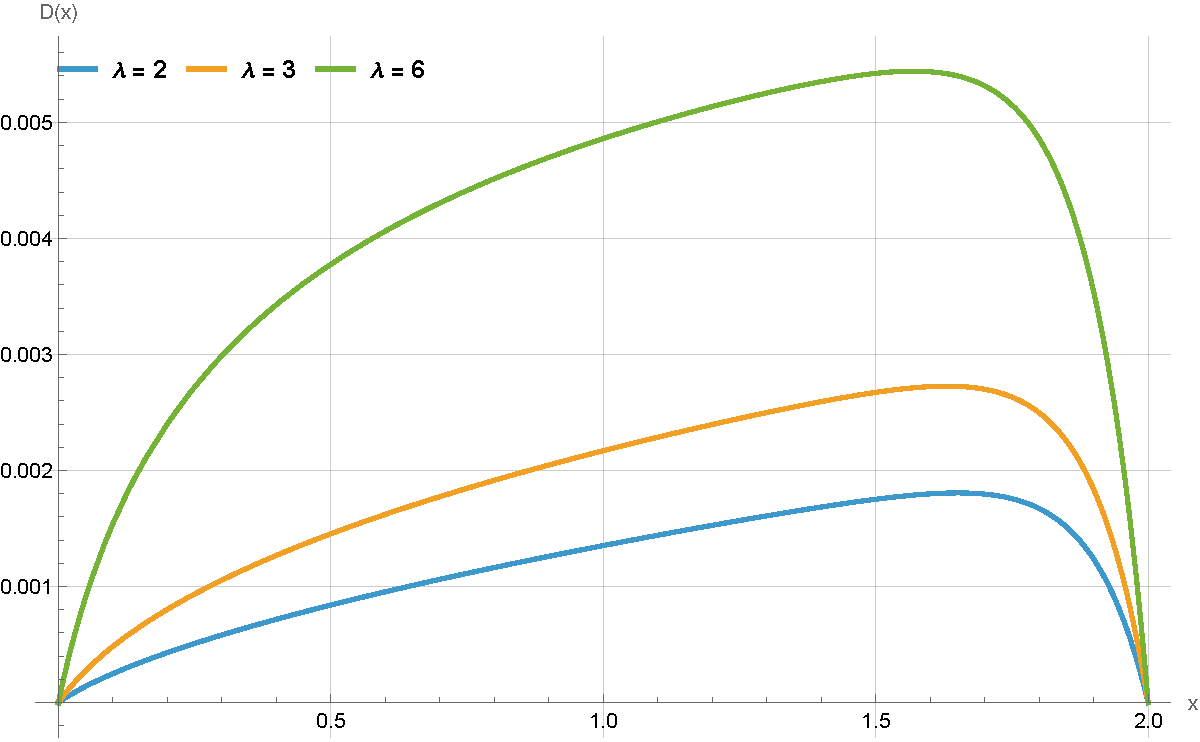
\includegraphics[width=\linewidth]{img/validation/Ovs/overshoot_lambda.pdf}
        \caption{Sensibilité de la fréquence des sauts $\lambda,\;\forall\;\lambda\in\{2,3,6\}$}\label{fig:Overshoot_lambda_visualisation}
    \end{subfigure}
    \hfill
    \begin{subfigure}{0.45\linewidth}
        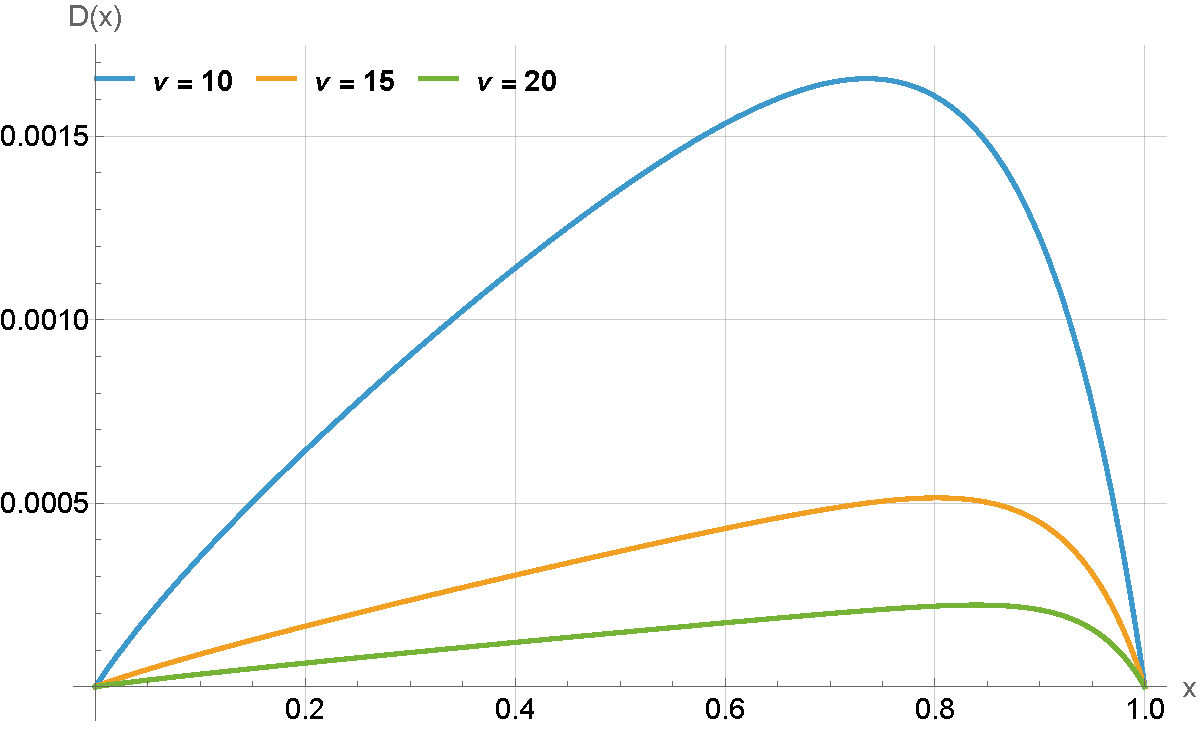
\includegraphics[width=\linewidth]{img/validation/Ovs/overshoot_nu.pdf}
        \caption{Sensibilité de la taille des sauts $\nu,\;\forall\;\nu\in\{5,10,15\}$}\label{fig:Overshoot_nu_visualisation}
    \end{subfigure}
    \hfill
    \caption{Visualisation de la fonction Dépassement Moyen $D(x)$}\label{fig:OvershootVisualisation}
\end{figure}
\FloatBarrier\paragraph{Analyse}\phantom{}\\
Les différents points suivants sont relevés:
\begin{itemize}
    \item Les conditions aux limites $D(0)=D(c)=0$ sont respectées;
    \item La fonction représente un \textit{dépassement moyen}, elle doit donc être positive pour toute valeur $x$ dans $[0,c]$;
    \item Une augmentation de la fréquence des sauts $\lambda$ induit une augmentation du dépassement moyen. En effet, il devient plus probable que le processus effectue un saut juste avant d'atteindre la frontière, ce qui augmente les chances de la franchir avec un certain excès.
    \item Une réduction de la taille des sauts (traduite par une augmentation de $\nu$) induit une diminution du dépassement moyen. En effet, même si un saut survient à proximité de la frontière, sa faible amplitude limite la distance franchie au-delà de celle-ci.
\end{itemize}

